\chapter{Object Recognition}
\label{cha:objrecog}

\begin{chapterabstract}
In this chapter, we address the problem of object class recognition. To approach this challenge, we rely on the geometric information provided by 3D object representations such as point clouds. Furthermore, we focus on learning-based methods to distinguish objects from different classes while capturing the variability of shape of different objects which belong to the same class. More specifically, we leverage deep learning for such task. The chapter begins introducing and formulating the object recognition task in Section \ref{cha:objrecog:sec:introduction} followed by a review of the most relevant literature and datasets in Sections \ref{cha:objrecog:sec:relatedworks} and \ref{cha:objrecog:sec:datasets}. After that, we present our first proposal for 3D object recognition, namely PointNet, in Section \ref{cha:objrecog:sec:pointnet}. Later, PointNet is improved and thoroughly tested in adverse conditions with noise and occlusion throughout the study in Section \ref{cha:objrecog:sec:study}. Next, LonchaNet is introduced in Section \ref{cha:objrecog:sec:lonchanet} as the last iteration of our system that incorporates all the lessons learned by the previous work. Finally, Section \ref{cha:objrecog:sec:conclusion} draws conclusions and sets future lines of research.
\end{chapterabstract}

\section{Introduction}
\label{cha:objrecog:sec:introduction}

Object recognition is fundamental to computer vision and despite the progress achieved during the last years, it still remains a challenging area of research. Arguably, most of the interest in object recognition is due to its usefulness for robotics.

In that regard, recognizing objects is one of the problems that must be solved to achieve total visual scene understanding. Such deeper and better knowledge of the environment eases and enables the execution of a wide variety of more complex tasks. For instance, accurately recognizing objects in a room can be extremely useful for any robotic system that navigates within indoor environments. Due to the unstructured nature of those environments, autonomous robots need to do reasoning grounded in the dynamic real world. In other words, they need to understand the information captured by their sensors to perform tasks such as grasping, navigation, mapping, or even providing humans with information about their surroundings. Identifying the classes to which objects belong is one key step to enhance the aforementioned capabilities.

Despite the easy intuitive interpretation of the problem, its inherent difficulty can be misleading. We humans recognize numerous objects in difficult settings (e.g., different points of view, occlusion, or clutter) with little to no effort. However, approaching that problem is not that easy for a computer and taking into account all the possible settings and combinations of external factors renders this task a difficult one to solve efficiently and with high precision (which is often required in numerous application scenarios).

From a formal point of view, the object recognition task can be formulated as follows: given an image $\mathcal{I}^{H\times W}$ in which an object $\mathcal{O}$ appears, which can be either a gray-scale or RGB array of $W$ pixels in width and $H$ pixels in height, the goal is to predict the class of the object $\mathcal{L_O}$ from a set of $N$ predefined object classes $\mathcal{L} = \{\mathcal{L}_0, \mathcal{L}_1, ..., \mathcal{L}_{N-1}\}$.

Most of the classic literature of this topic tackled such problem by devising hand-crafted feature descriptors that are extracted on certain keypoints detected over the bidimensional image and later used either to compare them against pre-existing object descriptors in a database to match them to a certain class or either to feed them as input to a shallow machine learning architecture that learns to classify those descriptors to predict the class of the object that appears in the image. That paradigm shifted recently due to the success of deep learning architectures that are able to exploit their feature learning capabilities to avoid the need of hand engineering descriptors while achieving unprecedented accuracy levels. Furthermore, the adoption and spread of depth sensors has also added a literally new dimension to learn from to boost performance. The approaches introduced in this thesis are part of that cutting-edge trend that takes advantage of the additional geometric information facilitated by commodity range scanners to perform learning over them using deep architectures. A more detailed review of the field, from the very beginning to the current trends using 3D data and deep neural networks, is performed in Section \ref{cha:objrecog:sec:relatedworks}.

After that literature review, we start describing our first approach to perform object recognition using 3D data, namely PointNet, capable of learning object classes from point clouds discretized as occupancy grids with uniform voxel grids in the tridimensional space. Section \ref{cha:objrecog:sec:pointnet} describes this architecture, its data representation, and also benchmarks it on a standard 3D object classification dataset (ModelNet) to validate it.

Following that, Section \ref{cha:objrecog:sec:study} analyzes how noise and occlusion impact such 3D deep learning architecture and the importance of the data representation when dealing with such adverse conditions that commonly appear in the real world. In that study, we also propose minor changes to the architecture and the representation themselves that significantly boost accuracy with regard to the originally proposed PointNet.

At last, Section \ref{cha:objrecog:sec:lonchanet} takes all the lessons learned from the initial PointNet proposal and the extensive study to introduce a novel slice-based architecture to tackle the 3D object class recognition problem, LonchaNet, which achieved state of the art results in the aforementioned benchmark (ModelNet10).

\section{Related Works}
\label{cha:objrecog:sec:relatedworks}

\subsection{2D Object Recognition}
\label{cha:objrecog:sec:relatedworks:subsec:2d}

\subsection{RGB-D Object Recognition}
\label{cha:objrecog:sec:relatedworks:subsec:rgbd}

\subsection{3D Object Recognition}
\label{cha:objrecog:sec:relatedworks:subsec:3d}

\section{Datasets}
\label{cha:objrecog:sec:datasets}

% TODO: Introductory paragraph

In order to evaluate the performance of our proposal in terms of accuracy we made extensive use of a well-known dataset such as the Princeton ModelNet project [REF]. Its goal, as their authors state, is to provide researchers with a comprehensive clean collection of 3D \ac{CAD} models for objects, which were obtained via online search engines. Employees from the Amazon Mechanical Turk service were hired to classify over $150,000$ models into $662$ categories.

At the moment, there are two versions of this dataset publicly available for download 2 : ModelNet-10 and ModelNet-40. Those are subsets of the original dataset, only providing the $10$ and $40$ most popular object categories respectively. They are specially clean since the models that did not belong to the specified categories were manually deleted.

On the one hand, ModelNet-10 is composed of a collection of over $5,000$ \ac{CAD} models classified into $10$ categories and divided into training and test sets. In addition, the orientation of all the \ac{CAD} models was manually aligned. On the other hand ModelNet-40 features over $9,800$ models classified into $40$ categories and it also includes training and test splits; however, their orientations are not aligned as they are in ModelNet-10.

\section{PointNet}
\label{cha:objrecog:sec:pointnet}

The proposed system takes a point cloud of an object as an input and predicts its class label. In this regard, the proposal is twofold: a volumetric grid based on point density to estimate spatial occupancy inside each voxel, and a pure \ac{3D}-\ac{CNN} which is trained to predict object classes. The occupancy grid -- inspired by VoxNet \cite{Maturana2015} occupancy models based on probabilistic estimates -- provides a compact representation of the object's 3D information from the point cloud. That grid is fed to the \ac{CNN} architecture, which in turn computes a label for that sample, i.e., predicts the class of the object.

\subsection{Data Representation}
\label{cha:objrecog:sec:pointnet:subsec:data}

As we mentioned before, our proposed architecture takes a point cloud of an object as input to recognize it. However, point clouds are unstructured representations that cannot be easily handled by common \ac{CNN} architectures due to the lack of a matrix-like organization. The most straightforward way to apply formal convolutions to that unstructured space is to impose a certain organization into it.

Occupancy grids are data structures which allow us to obtain a compact representation of the volumetric space. They stand between meshes or clouds, which offer rich but large amounts of information, and voxelized representations with packed but poor information. At that midpoint, occupancy grids provide considerable shape cues to perform learning, while enabling an efficient processing of that information thanks to their array-like implementation.


As we previously reviewed in Section \ref{cha:objrecog:sec:relatedworks}, certain 3D deep learning architectures make use of occupancy grids as a representation for the input data to be learned or classified. For instance, 3D ShapeNets \cite{Wu2015} is a \ac{CDBN} which represents a 3D shape as a $30 \times 30 \times 30$ binary tensor in which a one indicates that a voxel intersects the mesh surface, and a zero represents empty space. VoxNet \cite{Maturana2015} introduces three different occupancy grids ($32 \times 32 \times 32$ voxels) that employ 3D ray tracing to compute the number of beams hitting or passing each voxel and then use that information to compute the value of each voxel depending on the chosen model: a binary occupancy grid using probabilistic estimates, a density grid in which each voxel holds a value corresponding to the probability that it will block a sensor beam, and a hit grid that only considers hits thus ignoring empty or unknown space. The binary and density grids proposed by Maturana \emph{et al.} \cite{Maturana2015} differentiate unknown and empty space, whilst the hit grid and the binary tensor do not.

VoxNet’s occupancy grid outperforms 3D ShapeNets in terms of accuracy in the ModelNet challenge for the 3D-centric approaches described above. However, ray tracing grids considerably harmed performance in terms of execution time so that other approaches must be considered for a real-time implementation. In that very same work, the authors show that hit grids performed comparably to other approaches while keeping a low complexity to achieve a reduced runtime.

\begin{figure}[!t]
  \centering
  \begin{subfigure}{0.3\linewidth}
    \centering
    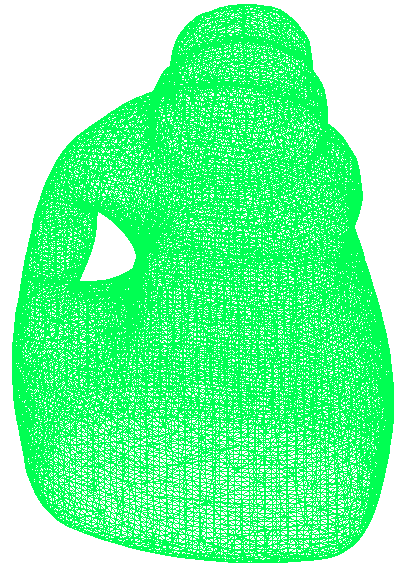
\includegraphics[width=\linewidth]{Figures/ObjRecog/detergent_mesh.png}
    \caption{Mesh}
    \label{fig:objrecog:meshcloudgrid:mesh}
  \end{subfigure}
  \begin{subfigure}{0.3\linewidth}
    \centering
    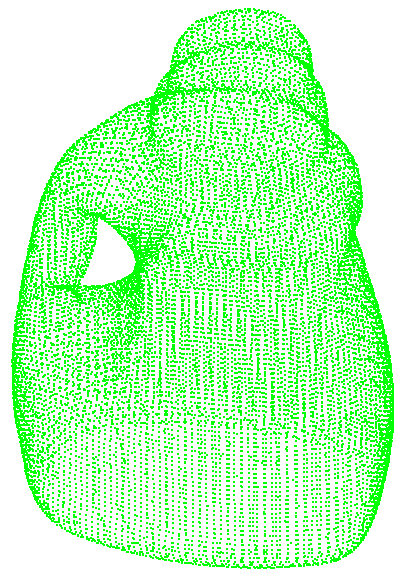
\includegraphics[width=\linewidth]{Figures/ObjRecog/detergent_cloud.png}
    \caption{Cloud}
    \label{fig:objrecog:meshcloudgrid:cloud}
  \end{subfigure}
  \begin{subfigure}{0.3\linewidth}
    \centering
    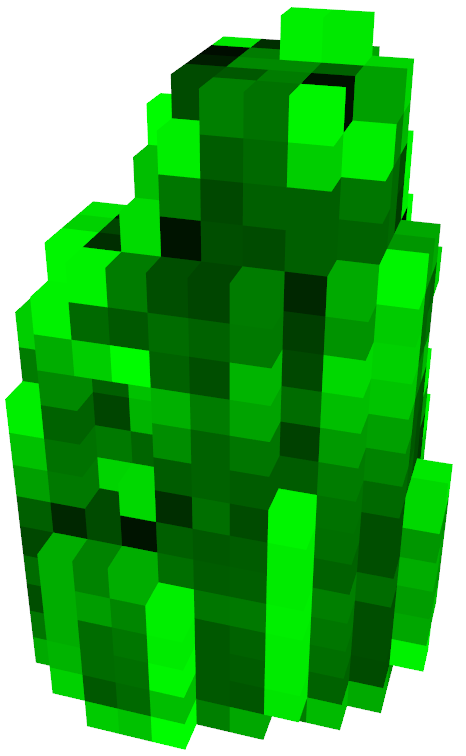
\includegraphics[width=0.9\linewidth]{Figures/ObjRecog/detergent_grid.png}
    \caption{Grid}
    \label{fig:objrecog:meshcloudgrid:grid}
  \end{subfigure}
  \caption{Various 3D representations for an object. A mesh (\subref{fig:objrecog:meshcloudgrid:mesh}) is transformed into a point cloud (\subref{fig:objrecog:meshcloudgrid:cloud}), and that cloud is processed to obtain a voxelized occupancy grid (\subref{fig:objrecog:meshcloudgrid:grid}). The occupancy grid shown in this figure is a cube of $30\times 30 \times 30$ voxels. Each voxel of that cube holds the point density inside its volume. In this case, dark voxels indicate high density whilst bright ones are low density volumes. Empty voxels were removed for better visualization.}
  \label{fig:objrecog:meshcloudgrid}
\end{figure}

With PointNet, we propose an occupancy grid inspired by the aforementioned successes but aiming to maintain a reasonable accuracy while allowing a real-time implementation. In our volumetric representation, each point of a cloud is mapped to a voxel of a fixed-size occupancy grid. Before performing that mapping, the object cloud is scaled to fit the grid. Each voxel will hold a value representing the number of points mapped to itself. At last, the values held by each cell are normalized. Figure \ref{fig:objrecog:meshcloudgrid} shows the derivation of the proposed occupancy grid representation from other typical tridimensional representations of a sample object.

\subsection{Network Architecture}
\label{cha:objrecog:sec:pointnet:subsec:network}

\begin{figure}[!t]
  \centering
  \includegraphics{example-image}
  \caption{PointNet's 3D \ac{CNN} architecture. [MISSINGDETAILS]}
  \label{fig:objrecog:pointnetarch}
\end{figure}

As we have previously stated, \acp{CNN} have proven to be very useful for recognizing and classifying objects in 2D images. A convolutional layer can recognize basic patterns such as corners or planes and if we stack several of them they can learn a topology of hierarchical filters that highlight regions of the images. What is more, the composition of several of these regions can define a feature of a more complex object. In this regard, a combination of various filters is able to recognize a full object. We apply this approach used in 2D images to 3D recognition. The deep architecture featured by PointNet is represented in Figure \ref{fig:objrecog:pointnetarch}. This setup allows PointNet to be on par with state-of-the-art algorithms while keeping reduced execution times.

\subsection{Experiments}
\label{cha:objrecog:sec:pointnet:subsec:experiments}

% TODO: Experiment details and procedure

\subsubsection{Data Generation}

\begin{figure}[!t]
  \centering
  \begin{subfigure}{\linewidth}
    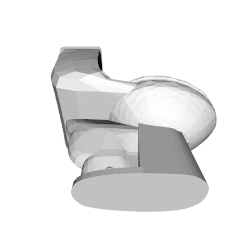
\includegraphics[width=0.24\linewidth]{Figures/ObjRecog/toilet_0}
    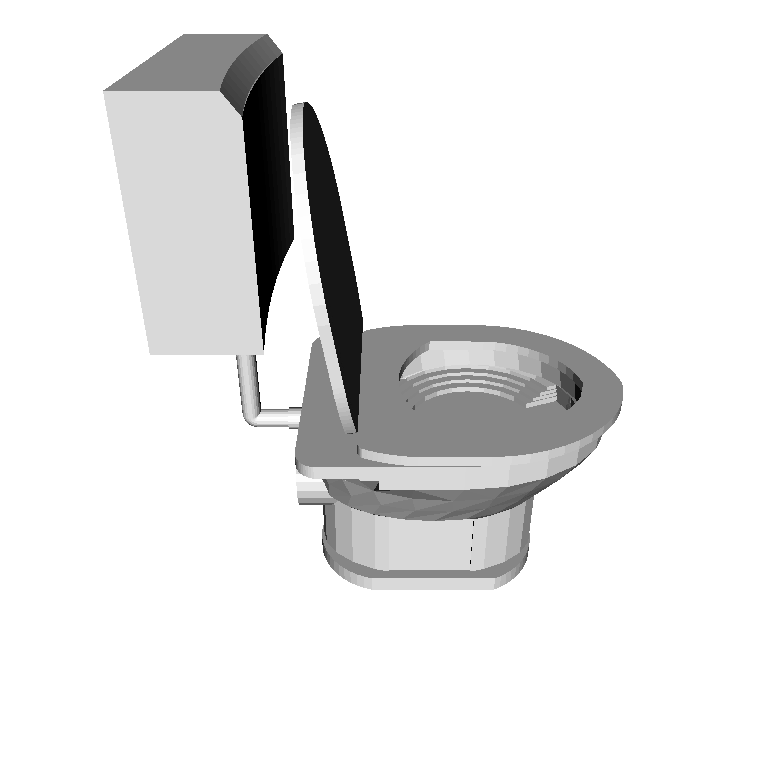
\includegraphics[width=0.24\linewidth]{Figures/ObjRecog/toilet_1}
    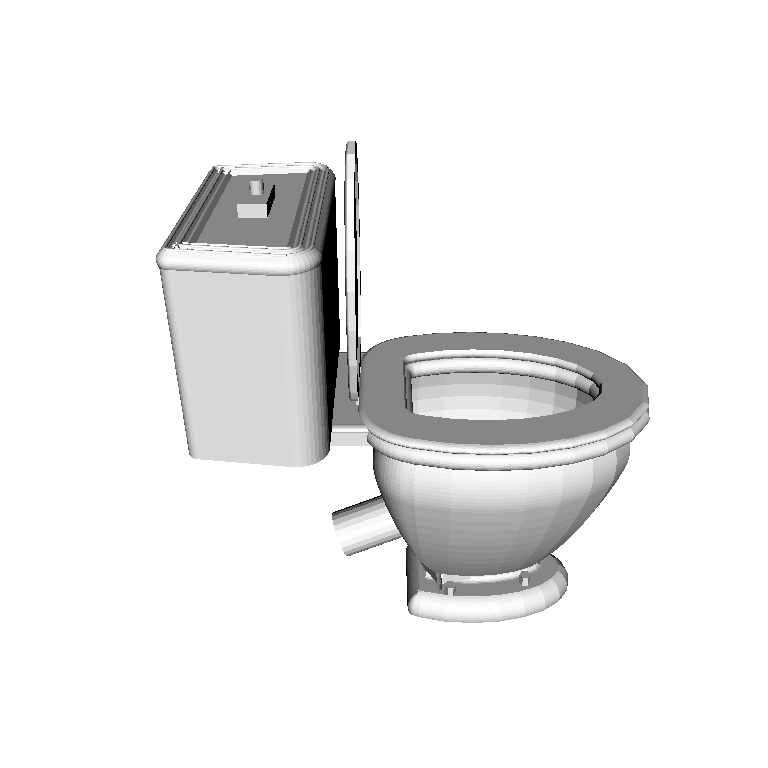
\includegraphics[width=0.24\linewidth]{Figures/ObjRecog/toilet_2}
    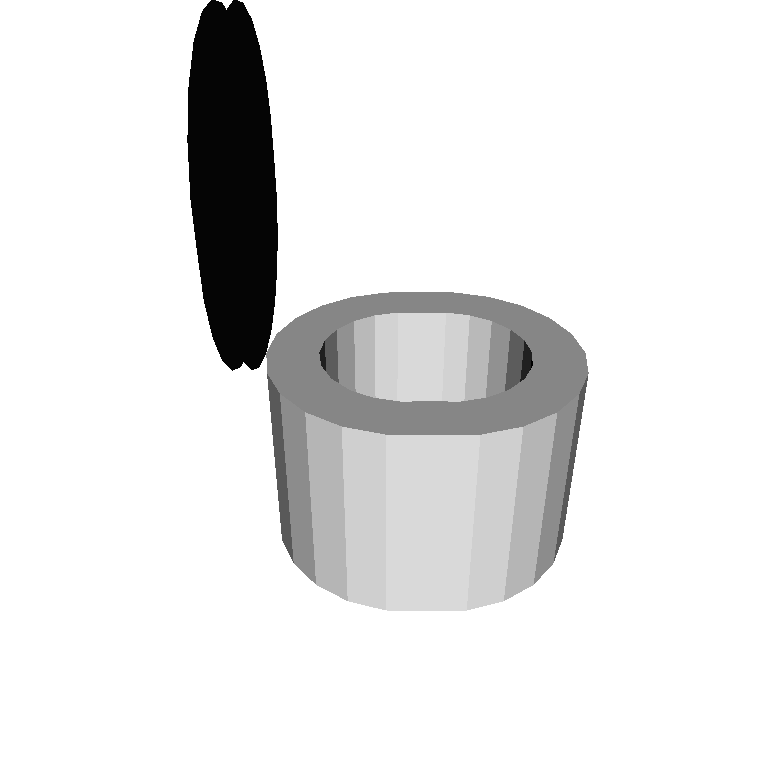
\includegraphics[width=0.24\linewidth]{Figures/ObjRecog/toilet_3}
    \caption{Rendered views.}
    \label{fig:objrecog:dataproc:renders}
  \end{subfigure}
  \begin{subfigure}{0.32\linewidth}
    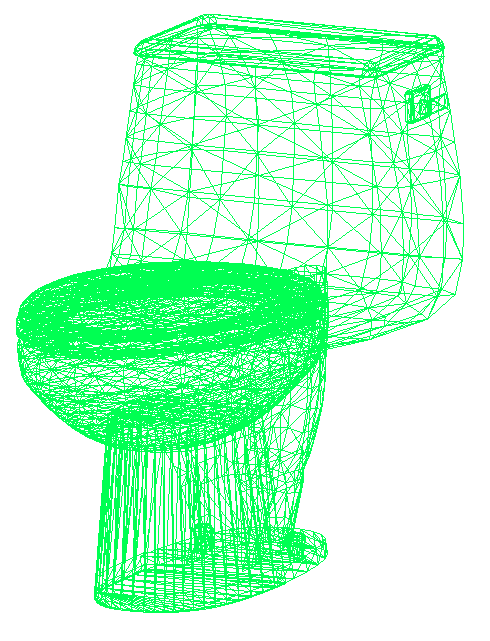
\includegraphics[width=\linewidth]{Figures/ObjRecog/toilet_off.png}
    \caption{Mesh.}
    \label{fig:objrecog:dataproc:mesh}
  \end{subfigure}
  \begin{subfigure}{0.32\linewidth}
    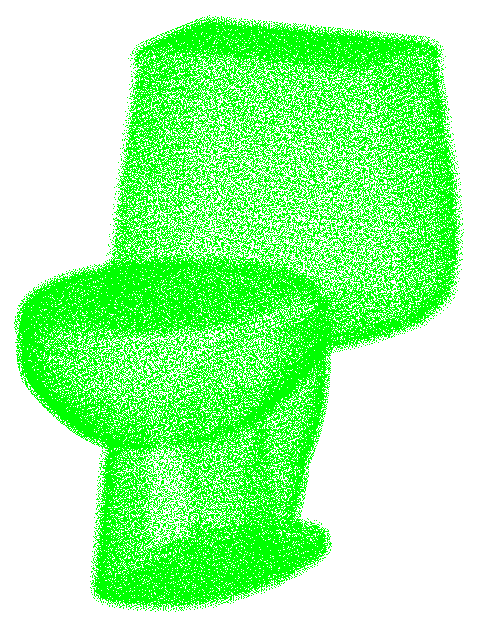
\includegraphics[width=\linewidth]{Figures/ObjRecog/toilet_cloud.png}
    \caption{Cloud.}
    \label{fig:objrecog:dataproc:cloud}
  \end{subfigure}
  \begin{subfigure}{0.32\linewidth}
    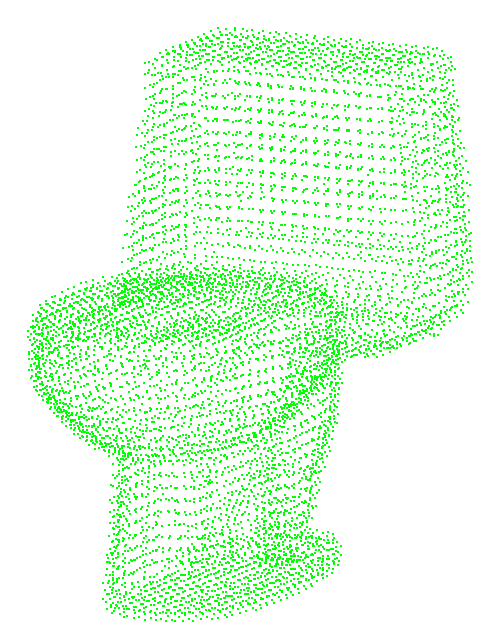
\includegraphics[width=\linewidth]{Figures/ObjRecog/toilet_cloud_downsampled.png}
    \caption{Downsampled.}
    \label{fig:objrecog:dataproc:downsampled}
  \end{subfigure}
  \caption{Dataset model processing example to generate the point clouds for PointNet. Some rendered views of a toilet model are shown in (\subref{fig:objrecog:dataproc:renders}). The original \ac{OFF} mesh is shown in (\subref{fig:objrecog:dataproc:mesh}). The generated point cloud after merging all points of view is shown in (\subref{fig:objrecog:dataproc:cloud}), and (\subref{fig:objrecog:dataproc:downsampled}) shows the downsampled cloud using a voxel grid filter with a leaf size of $0.7 \times 0.7 \times 0.7$.}
  \label{fig:objrecog:pointnetarch}
\end{figure}

The CAD models are provided in \ac{OFF}. Firstly, we converted all \ac{OFF} models into \ac{PLY} to ease the usage of the dataset with the \ac{PCL}. As we already mentioned, the input for PointNet are point clouds, but the dataset provides \ac{CAD} models specifying vertices and faces. In this regard, we converted the PLY models into \ac{PCD} clouds by raytracing them. A 3D sphere is tessellated and a virtual camera is placed in each vertex of that truncated icosahedron – pointing to the origin of the model – then multiple snapshots are rendered using raytracing and the z-buffer data, which contains the depth information, is used to generate point clouds from each point of view. After all points of view have been processed, the point clouds are merged. A voxel grid filter is applied to downsample the clouds after the raytracing operations. Figure 3 illustrates the aforementioned processes. After that, the resulting point clouds are used to train, randomizing the order of the models, and test the system taking into account the corresponding splits.

\subsubsection{Implementation}

This architecture was implemented using the \ac{PCL} \cite{Rusu2011}\cite{Aldoma2012} – which provides state-of-the-art algorithm implementations for 3D point cloud processing – and Caffe \cite{Jia2014}, a deep learning framework developed and maintained by the \ac{BVLC} and an active community of contributors on GitHub \footnote{\url{https://github.com/BVLC/caffe}}. This BSD-licensed C++ library enables researchers to design, train, and deploy \ac{CNN} architectures efficiently, mainly thanks to its drop-in integration of NVIDIA cuDNN \cite{Chetlur2014} to take advantage of \ac{GPU} acceleration.

% TODO: Source code

\subsubsection{Setup}

All the timings and results were obtained by performing the experiments in the following test setup: Intel Core i5-3570 with 8 GB of 1600 MHz DD3 RAM on an ASUS P8H77-M PRO motherboard (Intel H77 chipset). Additionally, the system includes an NVIDIA Tesla K20 GPU, and a Seagate Barracuda 7200.14 secondary storage. Caffe RC2 was run over ElementaryOS Freya 0.3.1, an Ubuntu-based Linux distribution. It was compiled using CMake 2.8.7, g++ 4.8.2, CUDA 7.0, and cuDNN v3.

\subsubsection{Results and Discussion}
\label{cha:objrecog:sec:pointnet:subsec:discussion}

As a result of training PointNet with a learning rate of 0.0001 and a momentum of 0.9 during 200 iterations using the ModelNet-10 dataset, it obtained a success rate of $77.6$\%. As shown in Figure [MISSINGREF], the confusion matrix reveals the stability of the system, mainly confusing items that look alike such as desk and table. Because of the nature of \acp{CNN}, which heavily rely on detecting combinations of features, these kind of errors are common. As we can observe in Figure \ref{fig:objrecog:tabledesk}, the visual features that define a desk and a table are almost the same, making it hard to distinguish between both classes. Figure \ref{fig:objrecog:tabledesk_activations} shows the neuron activations for the output layer of the architecture, proving that \emph{Desk} and \emph{Table} are consistently confused during the tests. In light of these experiments, and taking into account the knowledge of the \acp{CNN} principles, it is conceivable to think that a deeper network would provide better results so more experiments were carried out.

\begin{figure}
    \centering
    \begin{subfigure}{0.45\linewidth}
        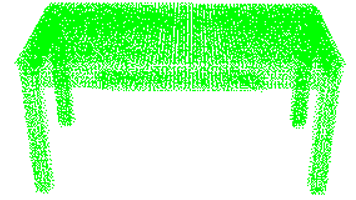
\includegraphics[width=\linewidth]{Figures/ObjRecog/table}
        \caption{}
        \label{subfig:objrecog:tabledesk:table}
    \end{subfigure}
    \begin{subfigure}{0.45\linewidth}
        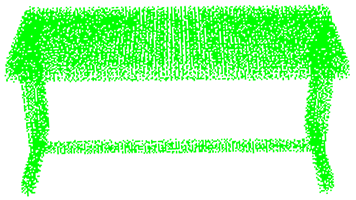
\includegraphics[width=\linewidth]{Figures/ObjRecog/desk}
        \caption{}
        \label{subfig:objrecog:tabledesk:desk}
    \end{subfigure}
    \caption{Similarity between two objects of different classes: Table and Desk. The point cloud shown in (\subref{subfig:objrecog:tabledesk:table}) represents an object of the Table class, whilst the point cloud in (\subref{subfig:objrecog:tabledesk:desk}) represents an object whose class is Desk but it is misclassified as a Table due to their resemblance.}
    \label{fig:objrecog:tabledesk}
\end{figure}

\begin{figure}
    \centering
    \begin{subfigure}{0.45\linewidth}
        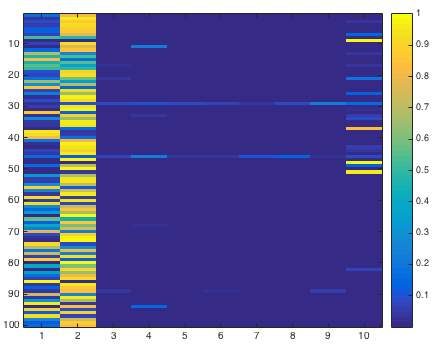
\includegraphics[width=\linewidth]{Figures/ObjRecog/table_matrix}
        \caption{}
        \label{subfig:objrecog:tabledesk_activations:table}
    \end{subfigure}
    \begin{subfigure}{0.45\linewidth}
        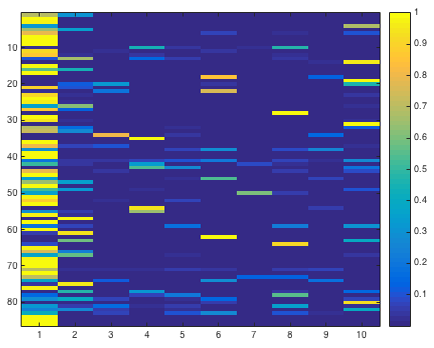
\includegraphics[width=\linewidth]{Figures/ObjRecog/desk_matrix}
        \caption{}
        \label{subfig:objrecog:tabledesk_activations:desk}
    \end{subfigure}
    \caption{Neuron activations for the output layer of the architecture when classifying all the test samples for both \emph{Desk}(\subref{subfig:objrecog:tabledesk_activations:desk}) and \emph{Table}(\subref{subfig:objrecog:tabledesk_activations:table}) classes. Each row represents an activation vector for a specific sample, so each column is a position of the vector: the activation to that particular class. The first column corresponds to the \emph{Desk} class, while the second one is the \emph{Table}. The activation shows the clear confusion between \emph{Desk} and \emph{Table}. Although the latter one is much less confused with other classes, many \emph{Tables} are misclassified as \emph{Desks} thus lowering the accuracy for this class.}
    \label{fig:objrecog:tabledesk_activations}
\end{figure}


In the deeper network experiment we added several layers to the PointNet architecture. One more convolutional layer was added since these layers are coupled to the detection of the features of the objects, so the more layers there are, a better or more expressive model is produced. An Inner Product layer was also added. Since these layers make the classification possible, adding more of them would theoretically provide better classification results.

This architecture was trained during $1,000$ iterations and tested every $200$ iterations. The best result was provided by the $800$ iterations test with an accuracy of $76.7$\%, while the $1,000$ iterations test dropped the performance to a $75.9$\% due to overfitting.

It is well known that training using an unbalanced dataset tends to harm those classes with the least number of examples and to benefit those with the most, as stated by [MISSINGREF]. Having this in mind, and knowing that ModelNet-10 is highly unbalanced as shown in Table [MISSINGTABLE], the dataset was balanced by limiting the number of examples of each class to $400$ using random undersampling. This does not fully solve the problem but improves the difference between the classes with the least number of examples and those with the most. The network was trained and tested with this more balanced dataset and it achieved an accuracy of $72.9$\%. The fact is that balancing the training set makes the accuracy of the classes with less examples higher, but it harms the success rate on classes with more, as seen in Figure \ref{fig:objrecog:balunbal}.

\begin{figure}[!htb]
    \centering
    \begin{tikzpicture}
        \begin{axis}[
            height=5cm,
            width=0.8\linewidth,
            ylabel=Accuracy,
            xlabel=Class,
            ymajorgrids=true,
            xtick pos=left,
            enlarge x limits=0.15,
            legend pos=outer north east,
            ybar=2pt,
            bar width=5 pt,
            xmin=1,
            xmax=10,
            ymin=0,
            ymax=1.0,
            ytick={0.0,0.1,...,1.1},
            xtick=data,
            axis on top=false,]
            \addplot [color=uagray80, fill=uablue50] coordinates {(1, 0.9) (2, 0.72) (3, 0.8) (4, 0.9) (5, 0.69) (6, 0.57) (7, 0.57) (8, 0.56) (9, 0.59) (10, 0.64)};
            \addplot [color=uagray80, fill=uablue10] coordinates {(1, 0.68) (2, 0.71) (3, 0.69) (4, 0.75) (5, 0.74) (6, 0.65) (7, 0.62) (8, 0.8) (9, 0.85) (10, 0.72)};
            \legend{Unbalanced, Balanced}
        \end{axis}
    \end{tikzpicture}
    \caption{Comparison of accuracy per class using an unbalanced dataset and a balanced one with a maximum of $400$ models per class via random undersampling. Accuracy is harmed in the classes in which models are removed but gained otherwise.}
    \label{fig:objrecog:balunbal}
\end{figure}

After analyzing the results, it can be stated that neither a deeper network nor balancing the dataset increase accuracy. In fact, the experiments of the original architecture with the unbalanced ModelNet-10 offered the best recognition results with a $77.6$\% success rate. In addition, PointNet featuring the architecture exposed in Figure [MISSINGREF] takes an average time of $24.6$ miliseconds to classify an example (in comparison with Voxnet, which can take up to half a second for its raytracing-based implementation). These results prove the system as a fast and accurate 3D object class recognition tool.

\subsection{Conclusion}
\label{cha:objrecog:sec:pointnet:subsec:conclusion}

PointNet is a brand new kind of CNN for object class recognition that handles tridimensional data, inspired by VoxNet and 3D ShapeNets but using density occupancy grids as inner representation for input data. It was implemented in Caffe and provides a faster method than the state of art ones yet obtaining a high success rate as the experiments over the ModelNet10 dataset. This fact enlightens a promising future in real-time 3D recognition tasks.

Following on this work, we plan to improve the inner representation by using adaptable occupancy grids instead of fixed-size ones. In addition, we will integrate the system in an object recognition pipeline for 3D scenes. Our network will receive a point cloud segment of the scene where the object lies, produced by a preprocessing method, and that segments will be used to generate the occupancy grids that will be learned by the system. This implies adapting the system for learning partial views of the objects and dealing with occlusions and scale changes. As an additional feature, we will include pose estimation in that pipeline, all of this with goal of developing an end-to-end 3D object recognition system.

\section{Noise and Occlusion}
\label{cha:objrecog:sec:study}

% TODO: Introductory text

\subsection{Data Representation}
\label{cha:objrecog:sec:study:subsec:representation}

As is clear from the previous sections, a volumetric representation to be fed to a \acs{2.5D} or \acs{3D}\acs{CNN} must encode the \acs{3D} shape of an object as a \acs{3D} tensor of binary or real values. This is due to the fact that raw \acs{3D} data is sparse, i.e., a \acs{3D} shape is only defined on its surface, and \acp{CNN} are not engineered for this kind of data.

In this regard, our proposal for the study is twofold. First, we implemented two different ways of generating the structure of the tensor -- position, grid size, and leaf size -- using a fixed grid and an adaptive one. Second, we developed two possible occupancy measures for the volumetric elements of the tensor.

\subsubsection{Tensor Generation}
\label{cha:objrecog:sec:study:subsec:representation:subsubsec:tensor}

Providing that the input to our network consists of point clouds generated from the information provided by \acs{RGB-D} sensors, we need to generate a discretized representation of the unbounded \acs{3D} data to feed the network. Each cloud will be represented as a \acs{3D} tensor. For that purpose, we need to spawn a grid to subdivide the space occupied by the point clouds. Two types are proposed: one with fixed leaf and grid sizes, and another one which will adapt those sizes to fit the data.

\paragraph{Fixed}

This kind of grid sets its origin at the minimum $x$, $y$, and $z$ values of the point cloud. Then the grid is spawned, with fixed and predefined sizes for both grid and voxels. After that, the cloud is scaled up or down to fit the grid. The scale factor is computed with respect to the dimension of maximum difference between the cloud and the grid. The cloud is scaled with that factor in all axes to maintain the original ratios. As a result, a cubic grid is generated as shown in Figure \ref{fig:objrecog:fixed}.

\begin{figure}[!ht]
	\centering
	\hfill
	\begin{subfigure}{0.325\textwidth}
		\centering
		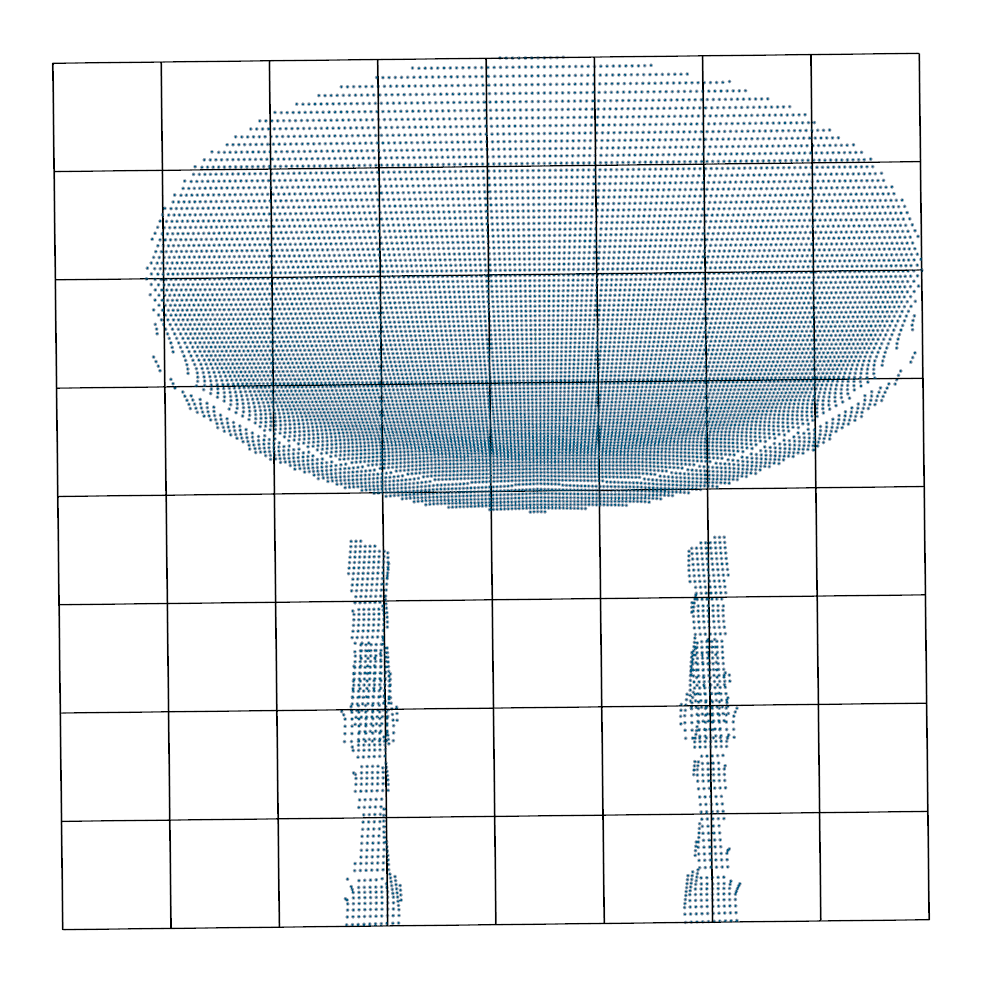
\includegraphics[width=\linewidth]{Figures/ObjRecog/fixed_front}
		\caption{Front}
		\label{subfig:objrecog:fixed:front}
	\end{subfigure}
	\hfill
	\begin{subfigure}{0.325\textwidth}
		\centering
		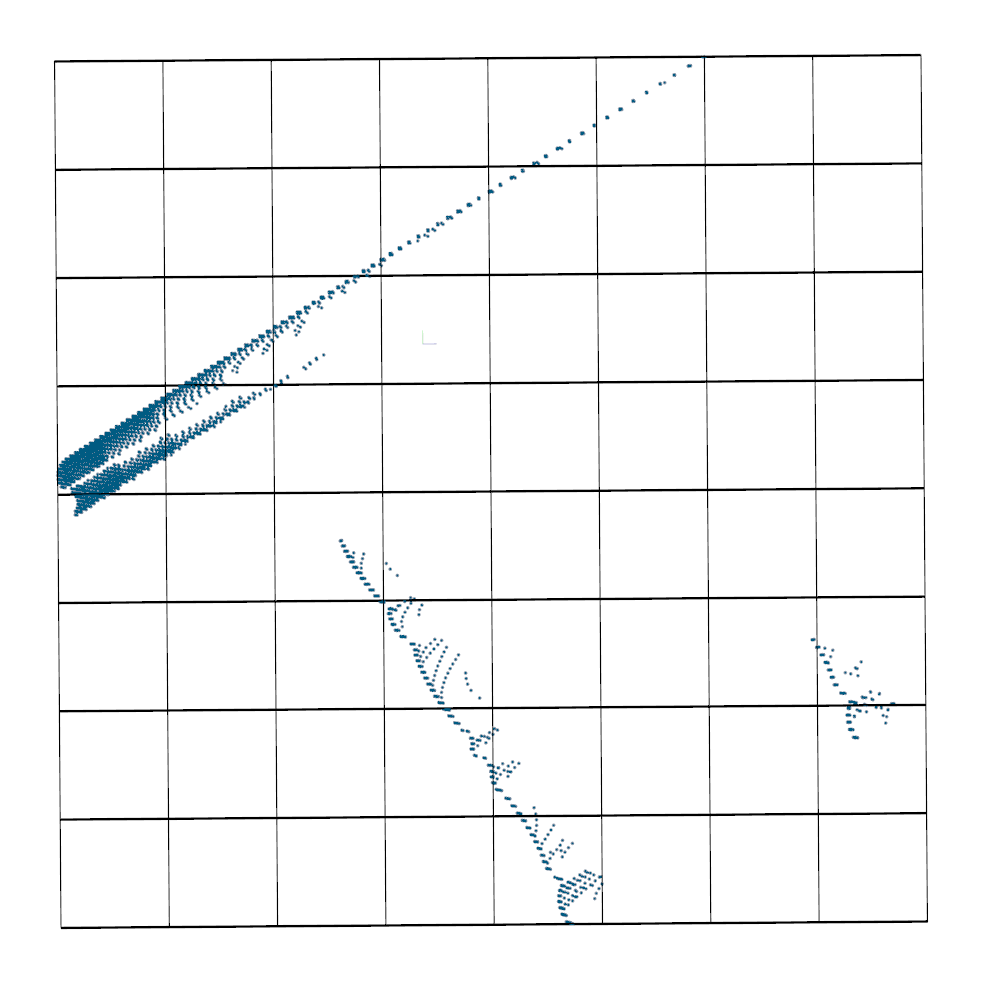
\includegraphics[width=\linewidth]{Figures/ObjRecog/fixed_side}
		\caption{Side}
		\label{subfig:objrecog:fixed:side}
	\end{subfigure}
	\hfill
	\begin{subfigure}{0.325\textwidth}
		\centering
		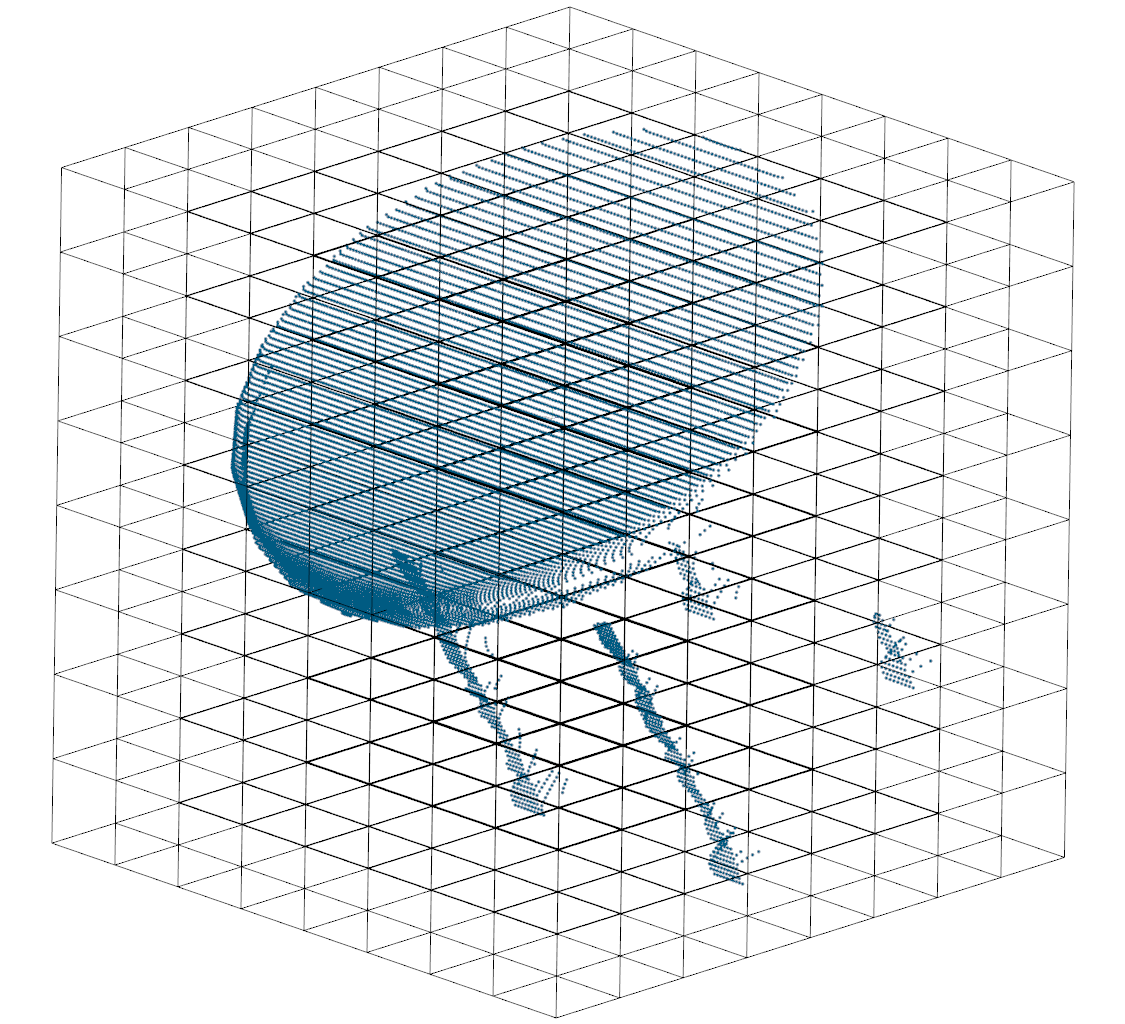
\includegraphics[width=\linewidth]{Figures/ObjRecog/fixed_persp}
		\caption{Perspective}
		\label{subfig:objrecog:fixed:persp}
	\end{subfigure}
	\hfill
	\caption{A fixed occupancy grid ($8\times8\times8$ voxels) with $40$ units leaf size and $320$ units grid size in all dimensions. The grid origin is placed at the minimum $x$, $y$, and $z$ values of the point cloud. Front (\subref{subfig:objrecog:fixed:front}), side (\subref{subfig:objrecog:fixed:side}), and perspective (\subref{subfig:objrecog:fixed:persp}) views of the grid over a partial view of a segmented table object are shown.}
	\label{fig:objrecog:fixed}
\end{figure}

\paragraph{Adaptive}

The adaptive grid also sets its origin at the minimum $x$, $y$, and $z$ values of the point cloud. Next, the grid size is adapted to the cloud dimensions. The leaf size is also computed in function of the grid size. Knowing both parameters, the grid is spawned, fitting the point cloud data. As a result, a non-cubic grid is generated. As shown in Figure \ref{fig:objrecog:adaptive}, all voxels have the same size, but they are not necessarily cubic.

\begin{figure}[!htb]
	\centering
	\hfill
	\begin{subfigure}{0.325\textwidth}
		\centering
		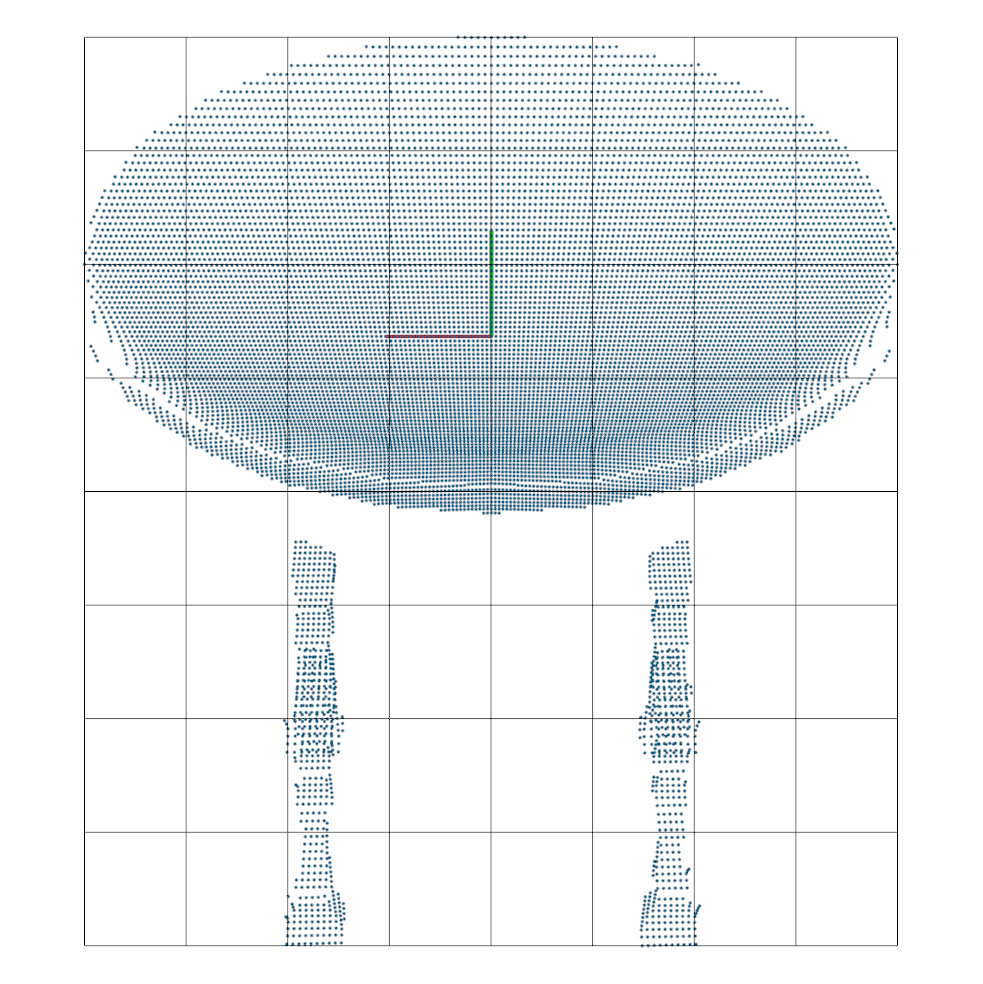
\includegraphics[width=\linewidth]{Figures/ObjRecog/adaptive_front}
		\caption{Front}
		\label{subfig:objrecog:adaptive:front}
	\end{subfigure}
	\hfill
	\begin{subfigure}{0.325\textwidth}
		\centering
		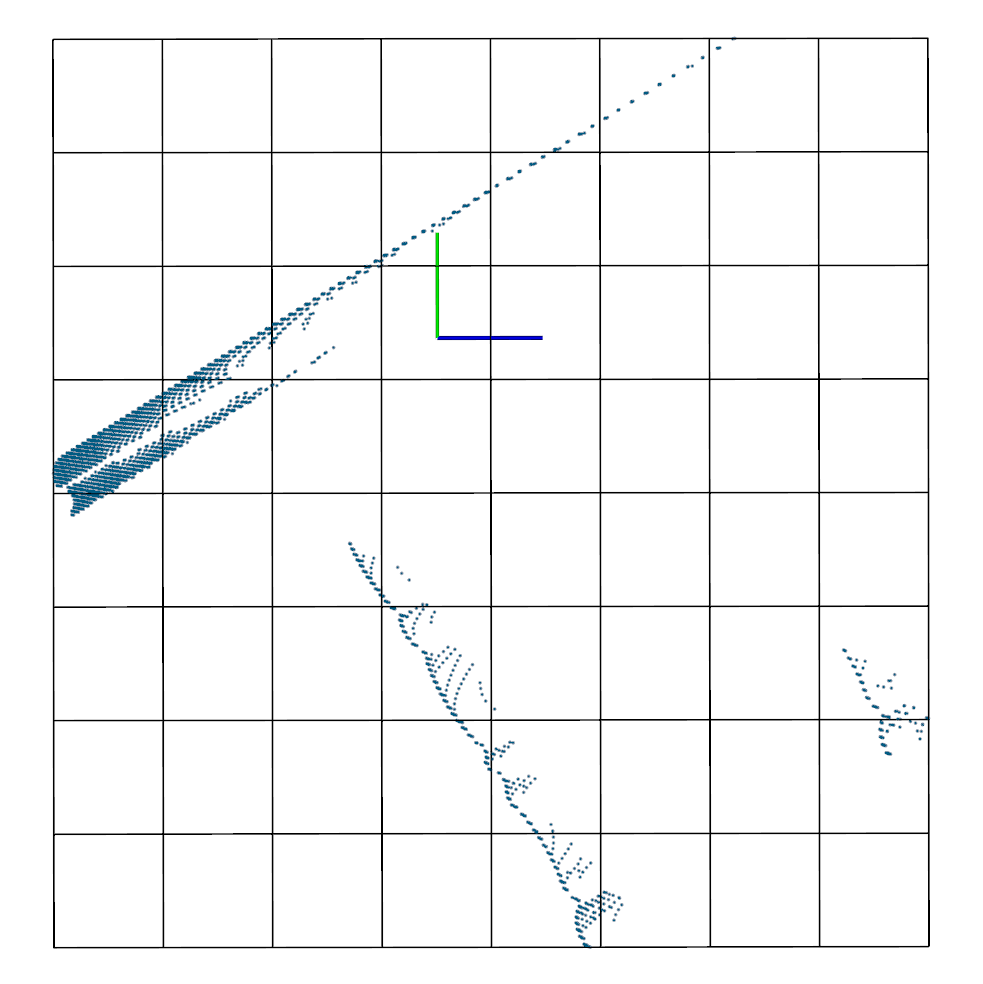
\includegraphics[width=\linewidth]{Figures/ObjRecog/adaptive_side}
		\caption{Side}
		\label{subfig:objrecog:adaptive:side}
	\end{subfigure}
	\hfill
	\begin{subfigure}{0.325\textwidth}
		\centering
		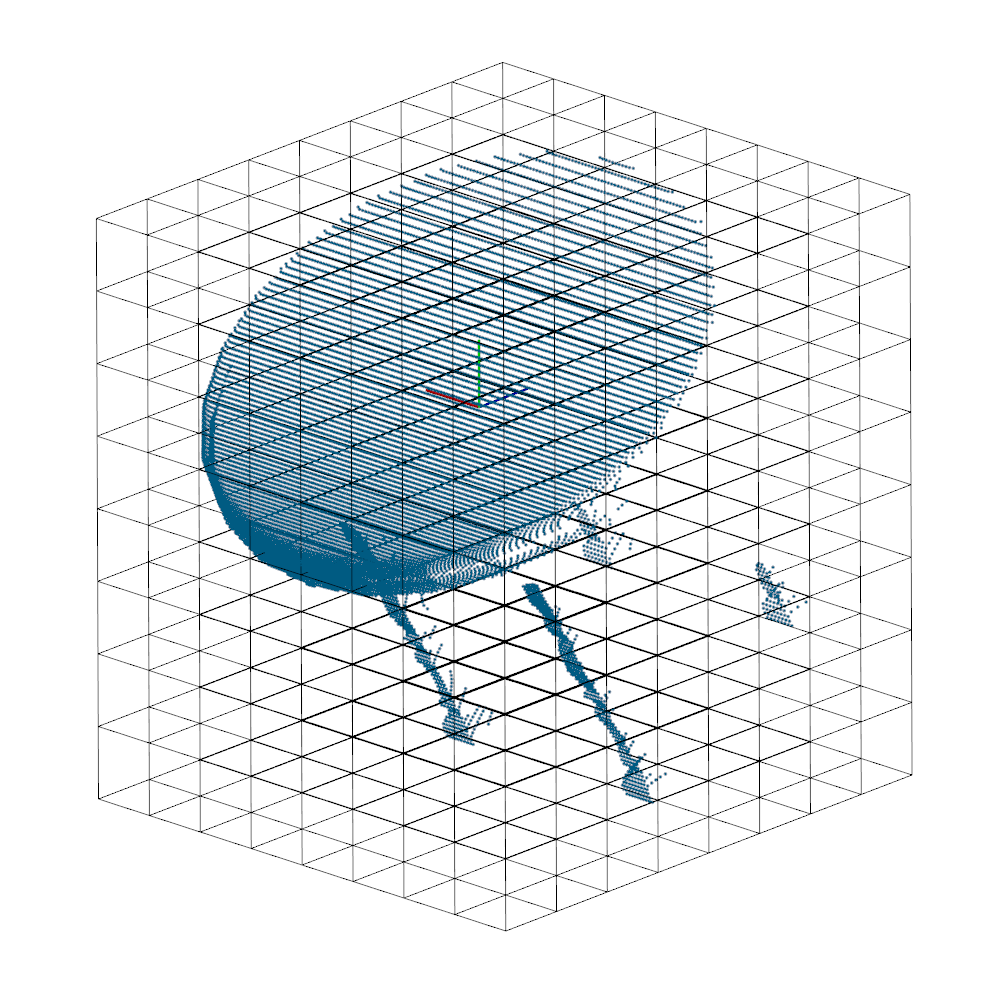
\includegraphics[width=\linewidth]{Figures/ObjRecog/adaptive_persp}
		\caption{Perspective}
		\label{subfig:objrecog:adaptive:persp}
	\end{subfigure}
	\hfill
	\caption{An adaptive occupancy grid ($8\times8\times8$ voxels) with adapted leaf and grid sizes in all dimensions to fit the data. The grid origin is placed at the minimum $x$, $y$, and $z$ values of the point cloud. Front (\subref{subfig:objrecog:adaptive:front}), side (\subref{subfig:objrecog:adaptive:side}), and perspective (\subref{subfig:objrecog:adaptive:persp}) views of the grid over a partial view of a segmented table object are shown. Notice that the point clouds for the three views are exactly the same for this figure and Figure \ref{fig:objrecog:fixed}, but the grids do change. There is a noticeable difference in the	front view. In Figure \ref{fig:objrecog:fixed}, using fixed grids, all voxels are cubic and the point cloud does not fit the grid completely (leftmost column in Figure \ref{subfig:objrecog:fixed:front}), whilst in this figure, with adaptive grids, the grid is fitted to the cloud.}
	\label{fig:objrecog:adaptive}
\end{figure}

It is important to remark that, in both cases (fixed and adaptive), the number of voxels in the grid is fixed. Figures \ref{fig:objrecog:fixed} and \ref{fig:objrecog:adaptive} show examples for both types using $8\times8\times8$ voxels for the sake of a better visualization.

It is also important to notice that each representation serves a purpose. The fixed grid will not always fit the data perfectly so it might end up having sparse zones with no information at all (as seen in Figure \ref{subfig:objrecog:fixed:front} on the first column). However, it can be used right away for sliding box detection. On the contrary, the adaptive grid fits the data to achieve a better representation. Nonetheless, it relies on a proper segmentation of the object to spawn the grid.

\subsubsection{Occupancy Computation}
\label{cha:objrecog:sec:study:subsec:representation:subsubsec:occupancy}

After spawning the grid to generate a discrete space, we need to determine the values for each cell or voxel of the \acs{3D} tensor. In order to do that, we must encode the geometric information of the point cloud into each occupied cell (see Figure \ref{fig:objrecog:grid_occ}). In other words, we have to summarize as a single value, the information of all points which lie inside a certain voxel. One way to do that is using occupancy measures. For that purpose, we propose two different alternatives: binary occupancy, normalized density.

\begin{figure}[!t]
	\centering
	\hfill
	\begin{subfigure}{0.325\textwidth}
		\centering
		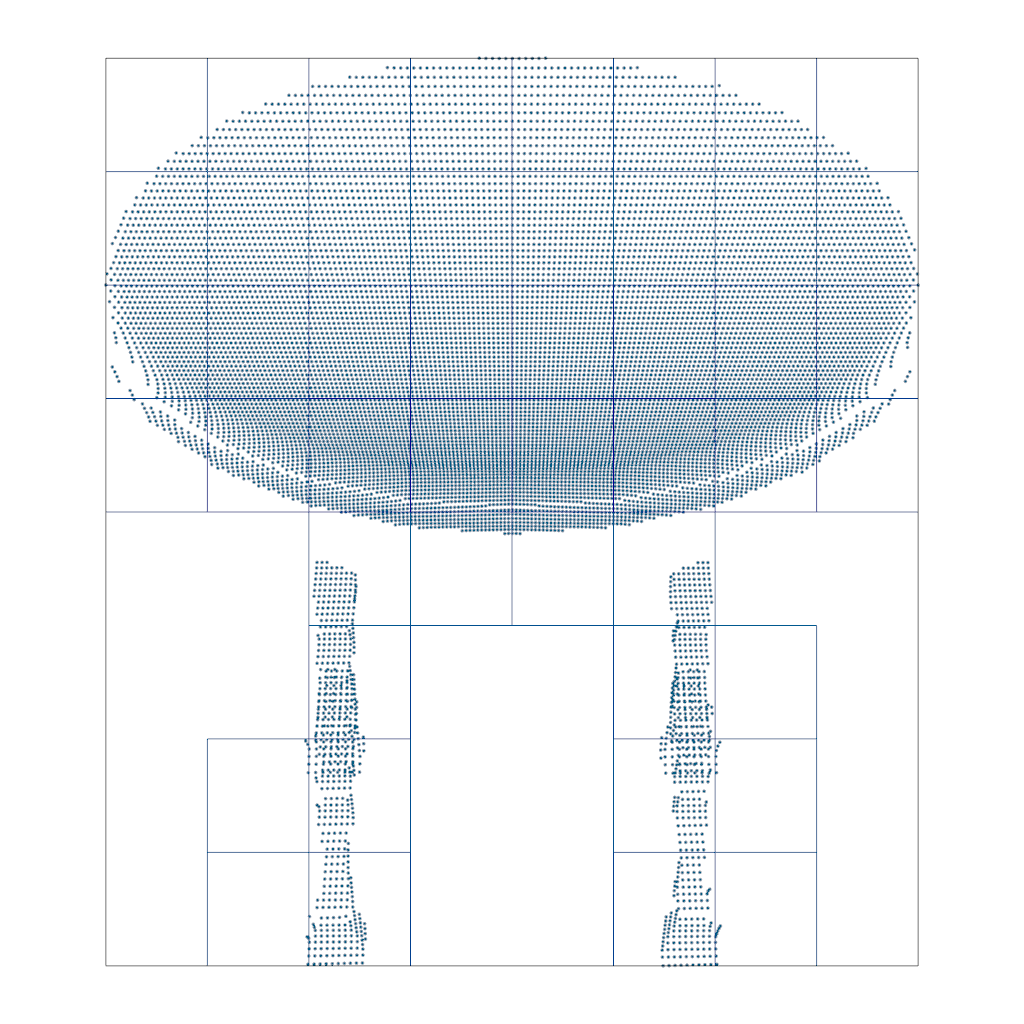
\includegraphics[width=\linewidth]{Figures/ObjRecog/surface_grid_front}
		\caption{Front}
		\label{subfig:objrecog:grid_occ:front}
	\end{subfigure}
	\hfill
	\begin{subfigure}{0.325\textwidth}
		\centering
		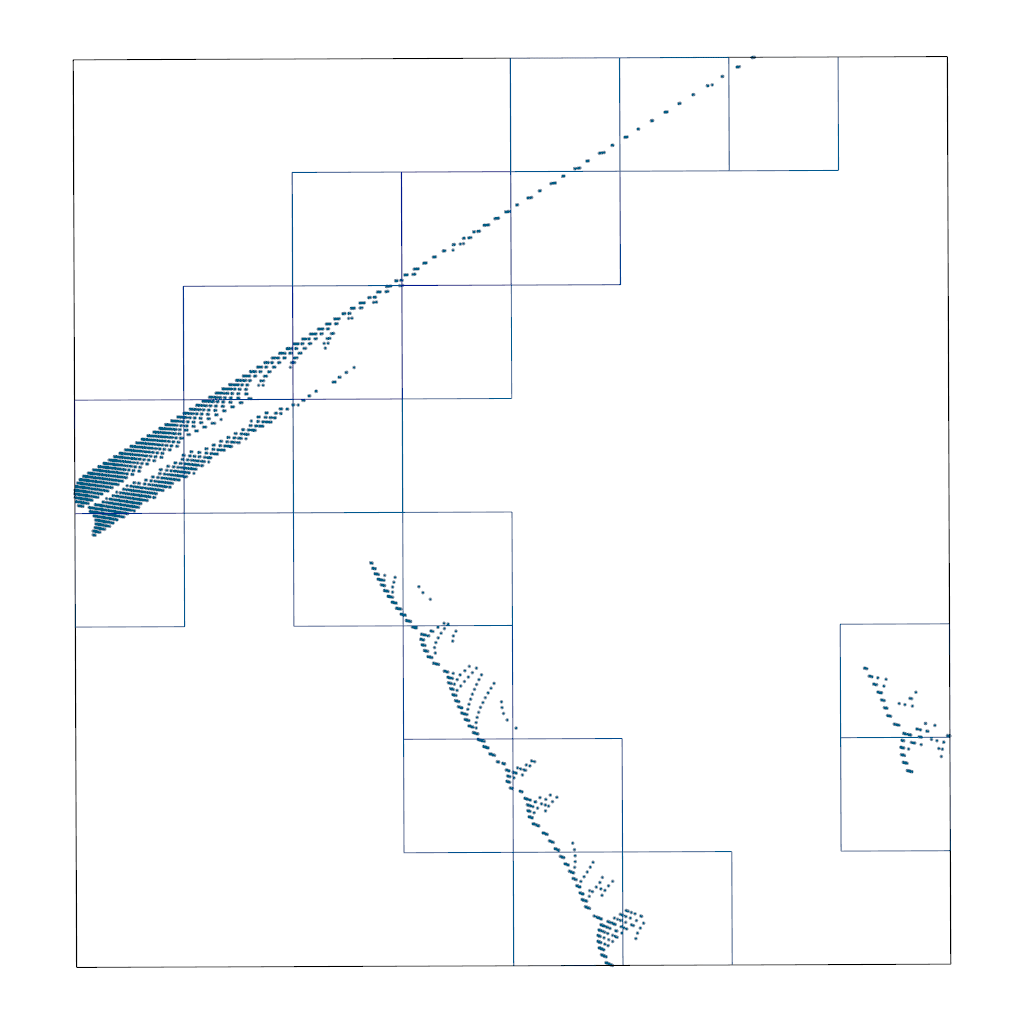
\includegraphics[width=\linewidth]{Figures/ObjRecog/surface_grid_side}
		\caption{Side}
		\label{subfig:objrecog:grid_occ:side}
	\end{subfigure}
	\hfill
	\begin{subfigure}{0.325\textwidth}
		\centering
		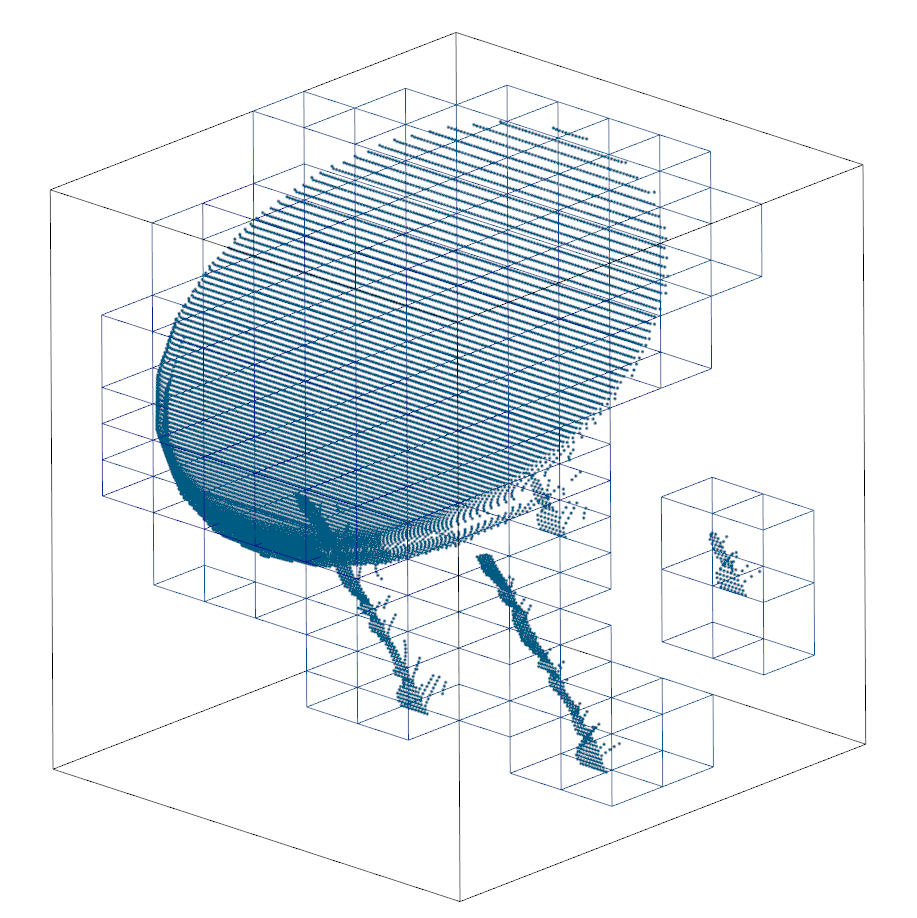
\includegraphics[width=\linewidth]{Figures/ObjRecog/surface_grid_persp}
		\caption{Perspective}
		\label{subfig:objrecog:grid_occ:persp}
	\end{subfigure}
	\hfill
	\caption{Occupied voxels in an adaptive $8\times8\times8$ grid generated over a partial view point cloud. Those voxels with points inside are shown in a wireframe representation. Empty voxels are omitted. Occupied voxels must be filled with values which represent the contained shape.}
	\label{fig:objrecog:grid_occ}
\end{figure}

\paragraph{Binary}

The binary tensor is the simplest representation that can be conceived to encode the shape. Voxels will hold binary values, they will be considered occupied if at least a point lies inside, and empty otherwise. Figure \ref{fig:objrecog:binary_occ} shows an example of this tensor.

\begin{figure}[!hb]
	\centering
	\hfill
	\begin{subfigure}{0.325\textwidth}
		\centering
		
\includegraphics[width=\linewidth]{Figures/ObjRecog/binary_front}
		\caption{Front}
		\label{subfig:objrecog:binary_occ:front}
	\end{subfigure}
	\hfill
	\begin{subfigure}{0.325\textwidth}
		\centering
		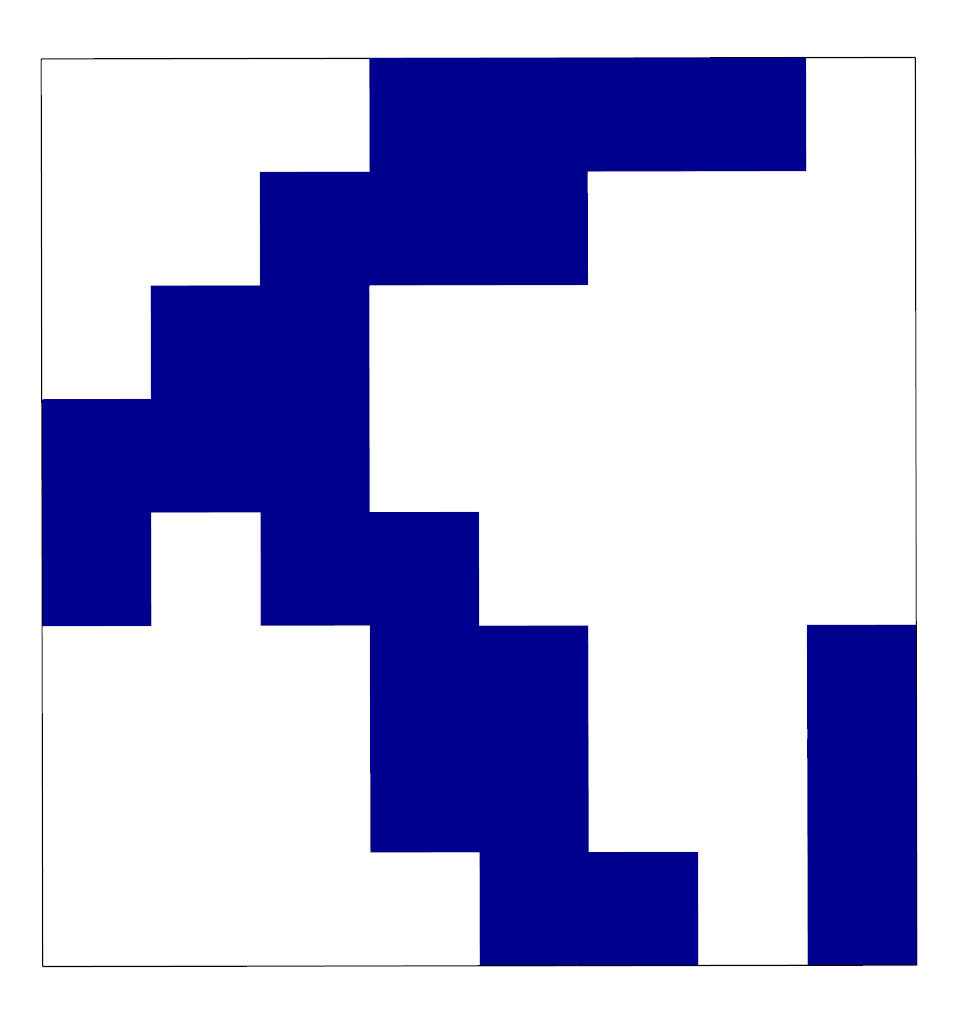
\includegraphics[width=\linewidth]{Figures/ObjRecog/binary_side}
		\caption{Side}
		\label{subfig:objrecog:binary_occ:side}
	\end{subfigure}
	\hfill
	\begin{subfigure}{0.325\textwidth}
		\centering
		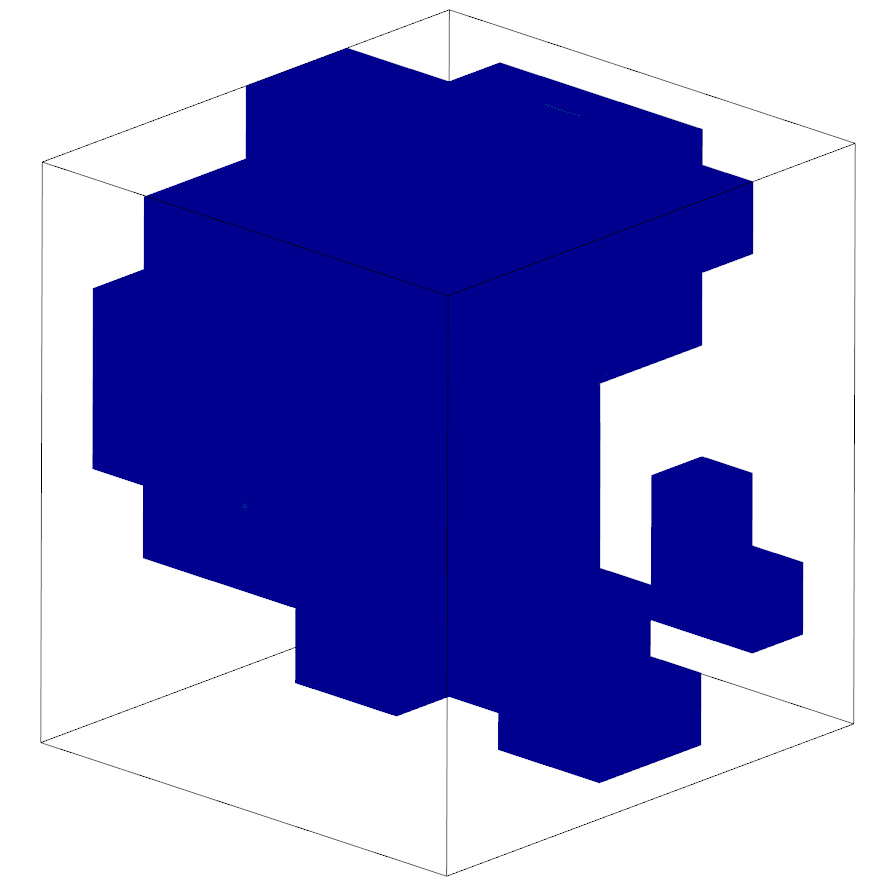
\includegraphics[width=\linewidth]{Figures/ObjRecog/binary_persp}
		\caption{Perspective}
		\label{subfig:objrecog:binary_occ:persp}
	\end{subfigure}
	\hfill
	\caption{Binary tensor computed over a point cloud of a partial view of an object (shown in Figure \ref{fig:objrecog:grid_occ}). Occupied voxels are shown in blue, empty voxels are omitted for the sake of simplicity.}
	\label{fig:objrecog:binary_occ}
\end{figure}

\paragraph{Normalized Density}

Binary representations are simple and require low computational power. However, complex shapes may get oversimplified so useful shape information gets lost. This representation can be improved by taking into account more shape information. A possible alternative consists of computing the point density inside each voxel, i.e., counting the number of points that fall within each cell.

It is important to notice that point density directly depends on the cloud resolution which in turn depends on many factors involving the camera and the scene, e.g., it is common for \acs{RGB-D} to generate denser shapes in closer surfaces. To alleviate this problem, we can normalize the density inside each voxel dividing each value by the maximum density over the whole tensor. An example of normalized density tensor is shown in Figure \ref{fig:objrecog:density_occ}.

\begin{figure}[!t]
	\centering
	\hfill
	\begin{subfigure}{0.325\textwidth}
		\centering
		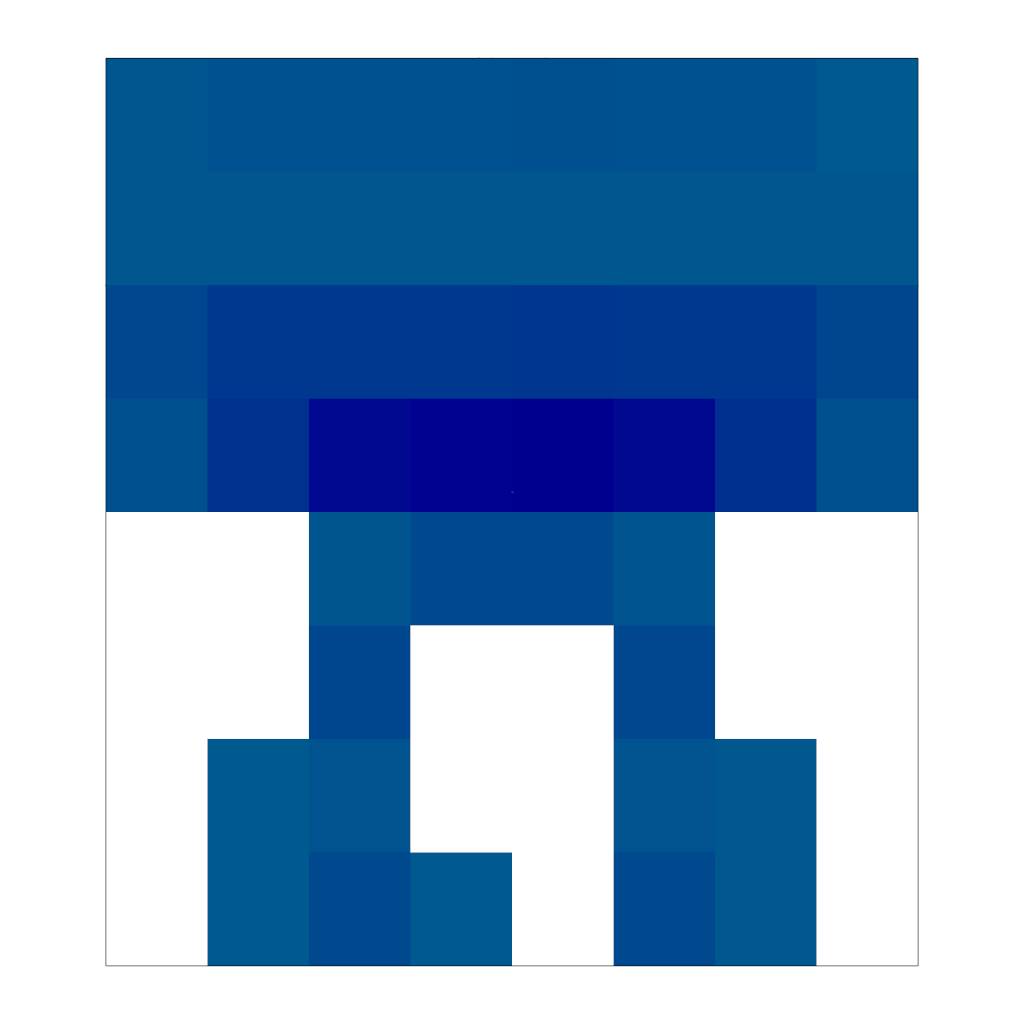
\includegraphics[width=\linewidth]{Figures/ObjRecog/density_front}
		\caption{Front}
		\label{subfig:objrecog:density_occ:front}
	\end{subfigure}
	\hfill
	\begin{subfigure}{0.325\textwidth}
		\centering
		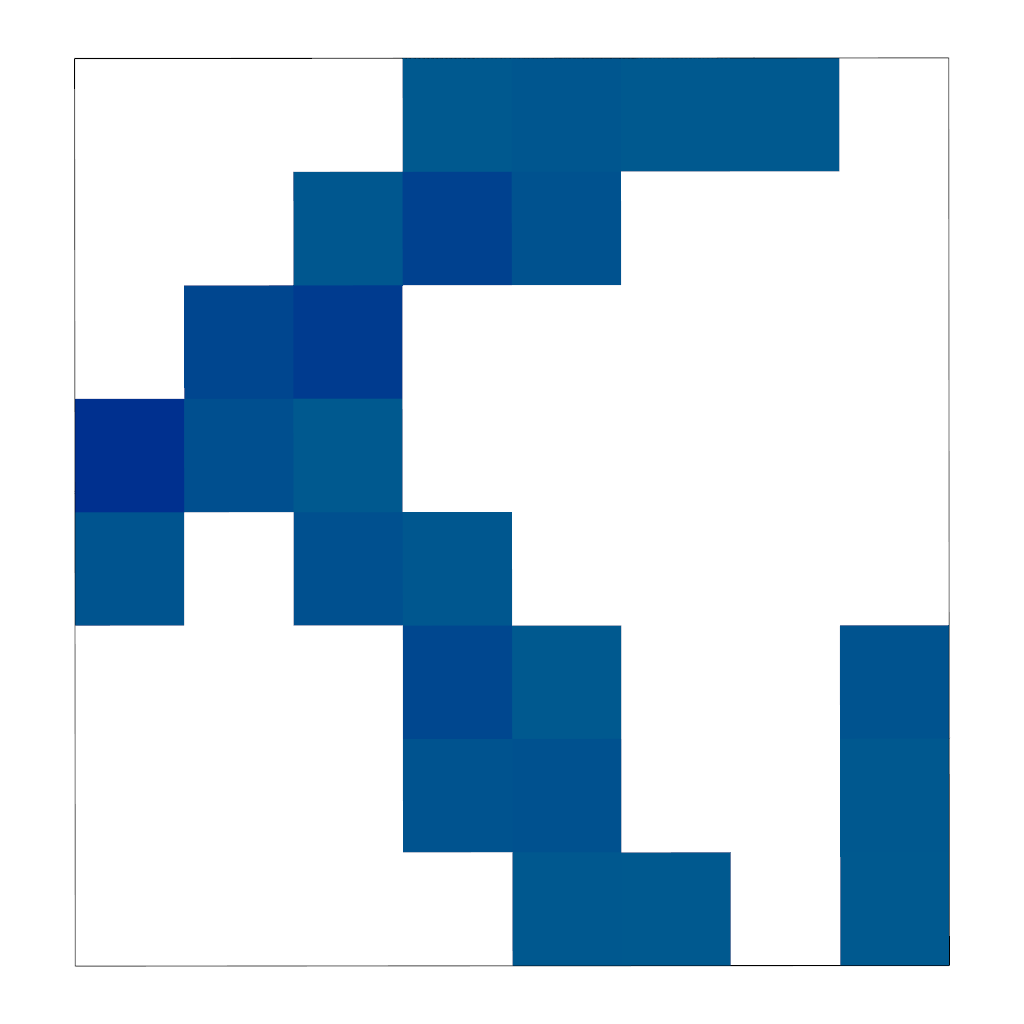
\includegraphics[width=\linewidth]{Figures/ObjRecog/density_side}
		\caption{Side}
		\label{subfig:objrecog:density_occ:side}
	\end{subfigure}
	\hfill
	\begin{subfigure}{0.325\textwidth}
		\centering
		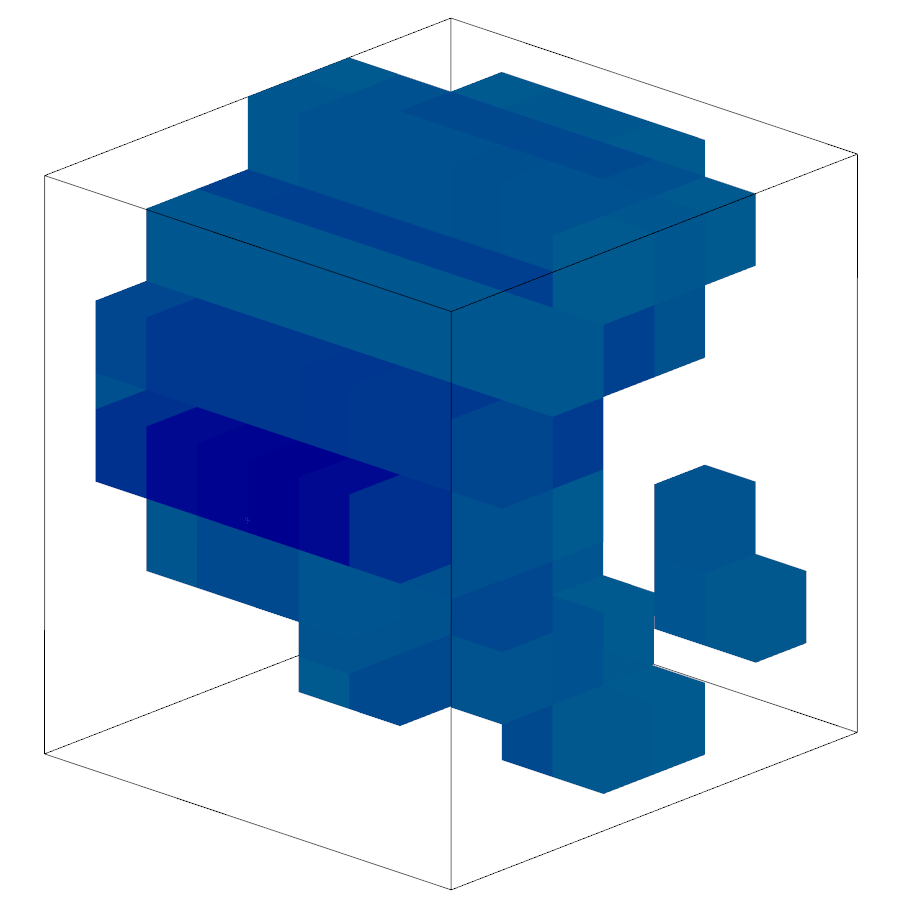
\includegraphics[width=\linewidth]{Figures/ObjRecog/density_persp}
		\caption{Perspective}
		\label{subfig:objrecog:density_occ:persp}
	\end{subfigure}
	\hfill
	\caption{Normalized density tensor over a point cloud of a partial view of an object (shown in Figure \ref{fig:objrecog:grid_occ}). Denser voxels are darker and sparse ones are shown in light blue. Empty voxels were removed for visualization purposes.}
	\label{fig:objrecog:density_occ}
\end{figure}

\subsection{Network Architecture}
\label{cha:objrecog:sec:study:subsec:architecture}

In this section, we will describe the main layers that compose the \ac{CNN} that will be used for the study. Figure \ref{fig:objrecog:cviuarch} shows a diagram of the chosen architecture. It is highly inspired by \emph{Voxnet} \cite{Maturana2015} and \emph{PointNet} \cite{Garcia-Garcia2016}. The network was implemented using Caffe. It features \acs{2D} convolutions and takes full \acs{3D} object model point clouds as input.

\begin{figure}[!b]
  \centering
  \includegraphics{example-image}
  \caption{CVIU's architecture. [MISSINGDETAILS]}
  \label{fig:objrecog:cviuarch}
\end{figure}

The input layer is a custom data layer implemented in Caffe which takes object point clouds as inputs and generates the corresponding discrete volumetric representation as discussed in the previous section.

Next, we can find a \emph{convolution layer} or $C(m, n, d)$. This layer applies $m$ filters of size $n\times n$ and a stride of $d\times d$ voxels. In our case, this first convolution layer learns $48$ $3\times3$ filters using a stride of $1\times 1$ voxels. This convolution layer is followed by a \ac{ReLU} activation to introduce non-linearities to the model.

After that, another convolution layer is found. In this case, it will learn $128$ $5\times5$ filters with a stride of $1\times 1$ voxels again. This layer is also followed by a \ac{ReLU} activation one.

A \emph{pooling layer} or $P(n, d)$ takes place after those blocks. It performs a max-pooling process to summarize the input data, taking the maximum value of a fixed local spatial region of $n\times n$ which is slided across the input volume using a stride of $d \times d$ voxels. In this case, a pooling region of $2\times 2$ voxels with the same stride was chosen.

At last, we can find an \emph{inner product layer} or $IP(n)$. It is just a fully connected layer, a traditional neural network architecture which consists of $n$ neurons ($1024$ in this case). It is followed by a \acs{ReLU} activation and a \emph{dropout layer} \cite{Srivastava2014} or $DP(r)$. The function of the dropout layer is to avoid overfitting, randomly dropping connections with a probability $r$ ($0.5$ in our case). In the end, another fully connected layer represents the output of the network, with as many output neurons as classes has our classification problem. Since our dataset has $10$ classes (see Section \ref{subsec:dataset}) this layer has $10$ neurons.

We use the term \acs{2.5D} to refer to this network due to the fact that it processes \acs{3D} data using \acs{2D} convolutions. This means that, in the end, its convolutions do not fully take into account the depth spatial dimension of the input as if we were using pure \acs{3D} convolution filters. It is intuitive to think that a \acs{3D} \acs{CNN} would yield better results due to that extra spatial dimension. However, a \acs{3D} \acs{CNN} has some disadvantages that made us consider using a \acs{2.5D} \acs{CNN} instead for the experimentation: (1) higher computational cost, (2) memory footprint is also much higher, (3) more parameters thus harder training. For those reasons, the main body of the experiments were carried out using the \acs{2.5D} approach.

\subsection{Experiments}
\label{cha:objrecog:sec:study:subsec:experiments}

In order to assess the performance of the proposed model-based \acs{CNN} we carried out an extensive experimentation to determine the accuracy of the model and its robustness against occlusions and noise -- situations that often occur in real-world scenes. For that purpose we started using the normalized density grids since they offer a good balance between efficiency and representation. We also investigated the effect of both fixed and adaptive grids using different sizes. Further experimentation was performed to compare the normalized density grids with the binary ones. We also carried out a brief experiment using a \acs{3D} \acs{CNN} to compare its performance with the \acs{2.5D} counterpart.

\subsubsection{Data Generation}
\label{cha:objrecog:sec:study:subsec:experiments:subsubsec:data}

\paragraph{Noise Simulation}

The partial views generated using the previously described process are not a good simulation of the result that we would obtain by using a low-cost \acs{RGB-D} sensor. Those systems are noisy, so the point clouds produced by them are not a perfect representation of the real-world objects.

In order to properly simulate the behavior of a sensor, a model is needed. In our case, we are dealing with low-cost \acs{RGB-D} sensors such as Microsoft Kinect and Primesense Carmine. A complete noise model for those sensors, specifically for the Kinect device, must take into account occlusion boundaries due to distance between the \ac{IR} projector and the \ac{IR} camera, $8$-bit quantization, $9\times9$ pixel correlation window smoothing, and $z$-axis or depth Gaussian noise \cite{Gschwandtner2011}.

We will make use of a simplification of this model, only taking into account the Gaussian noise since it is the most significant one for the generated partial views. In this regard, the synthetic views are augmented by adding Gaussian noise to the $z$ dimension of the point clouds with mean $\mu=0$ and different values for the standard deviation $\sigma$ to quantify the noise magnitude. Figure \ref{fig:objrecog:noise} shows the effect of this noise over a synthetic partial view of one object of the dataset.

\begin{figure}[!t]
	\centering
	\hfill
	\begin{subfigure}{0.32\textwidth}
		\centering
		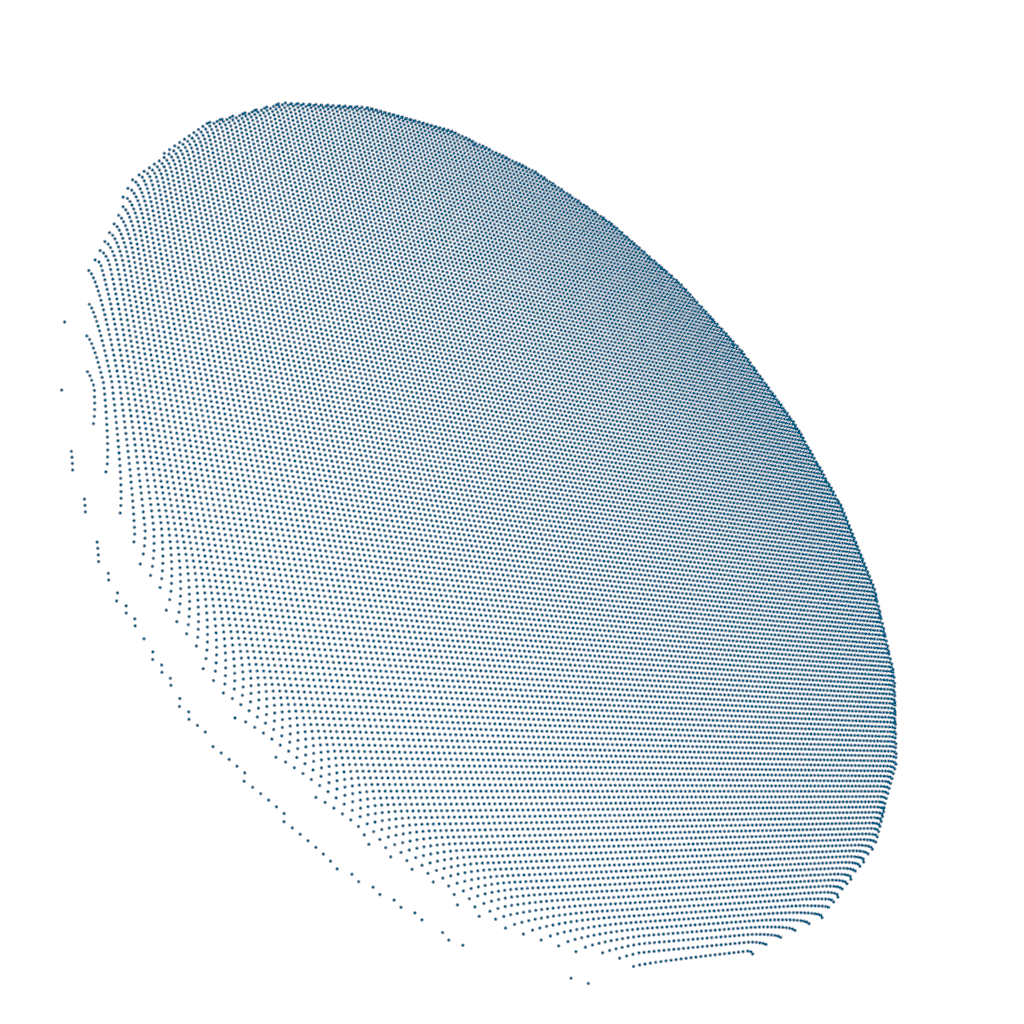
\includegraphics[width=\linewidth]{Figures/ObjRecog/stddev_0}
		\caption{$\sigma=0$}
		\label{subfig:objrecog:noise:0}
	\end{subfigure}
	\hfill
	\begin{subfigure}{0.32\textwidth}
		\centering
		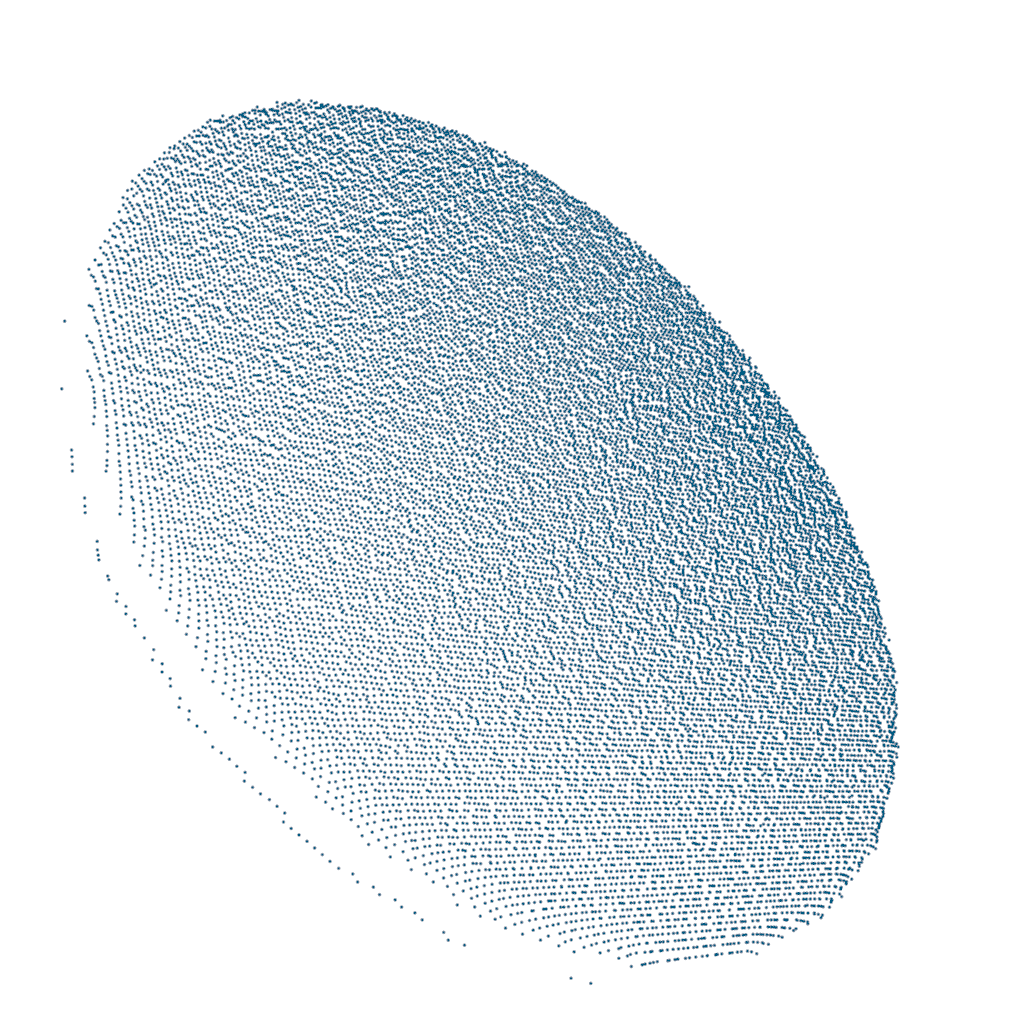
\includegraphics[width=\linewidth]{Figures/ObjRecog/stddev_01}
		\caption{$\sigma=0.1$}
		\label{subfig:objrecog:noise:01}
	\end{subfigure}
	\hfill
	\begin{subfigure}{0.32\textwidth}
		\centering
		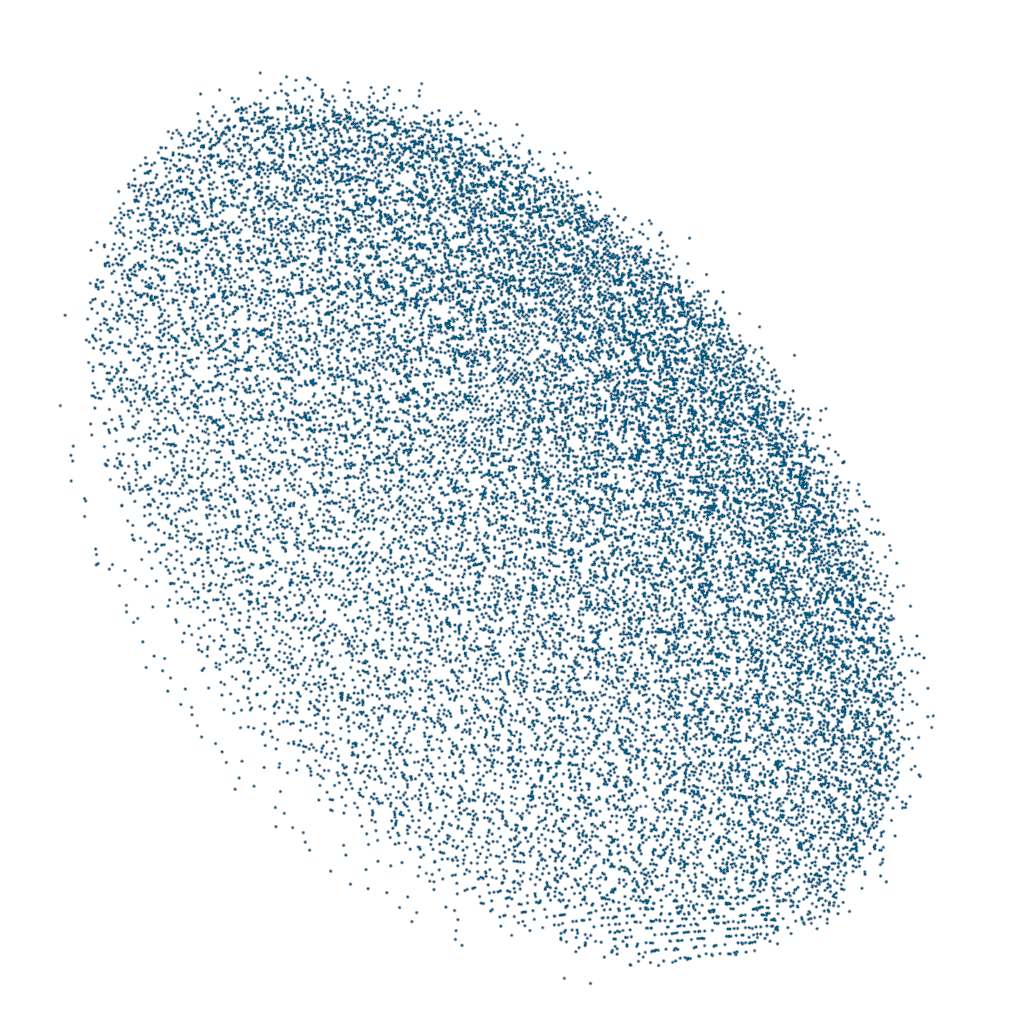
\includegraphics[width=\linewidth]{Figures/ObjRecog/stddev_1}
		\caption{$\sigma=1$}
		\label{subfig:objrecog:noise:1}
	\end{subfigure}
	\hfill
	\caption{Different levels of noise ($\sigma=0$ (\subref{subfig:objrecog:noise:0}), $\sigma=0.1$ (\subref{subfig:objrecog:noise:01}), and $\sigma=1$ (\subref{subfig:objrecog:noise:1})) applied to the $z$-axis of every point of a table partial view.}
	\label{fig:objrecog:noise}
\end{figure}

\paragraph{Occlusion Simulation}

In addition to modelling the sensor to improve our synthetic data, it is important to also take the environment into account. In a real-world scenario, objects are not usually perfectly isolated and easily segmented; in fact, it is common for them to be occluded by other elements of the scene.

The occlusion simulation process consists of picking a random point of the cloud with a uniform probability distribution. Then, a number of closest neighbors to that point are picked. At last, both the neighbors and the point are considered occluded surface and removed from the point cloud. The number of neighbors to pick depends on the amount of occlusion $\psi$ we want to simulate. For instance, for an occlusion $\psi=25\%$ we will remove neighbors until the rest of the cloud contains a $75\%$ of the original amount of points, i.e., we will remove a $25\%$ of the original cloud. Figure \ref{fig:occlusion} shows the effect of the random occlusion process with different occlusion factors $\psi$ over a synthetic partial view of a table object of the dataset.

It is important to notice the randomness of the occlusion process. This means that even with a high $\psi$ it is possible not to remove any important surface information and vice versa. In other words, it is possible for some objects to remove a $50\%$ of their points and still be recognizable because the removed region was not significant at all, e.g., a completely flat surface. However it is possible to render an object unrecognizable by removing a small portion of its points if the randomly picked surface is significant for its geometry. This remark is specially important when testing the robustness of the system. In order to guarantee that an appropriate measure of the robustness against missing information is obtained, a significant amount of testing sets must be generated and their results averaged so that it is highly probable to test against objects which have been occluded all over their surface across the whole testing set.

\begin{figure}[!t]
	\centering
	\hfill
	\begin{subfigure}{0.32\textwidth}
		\centering
		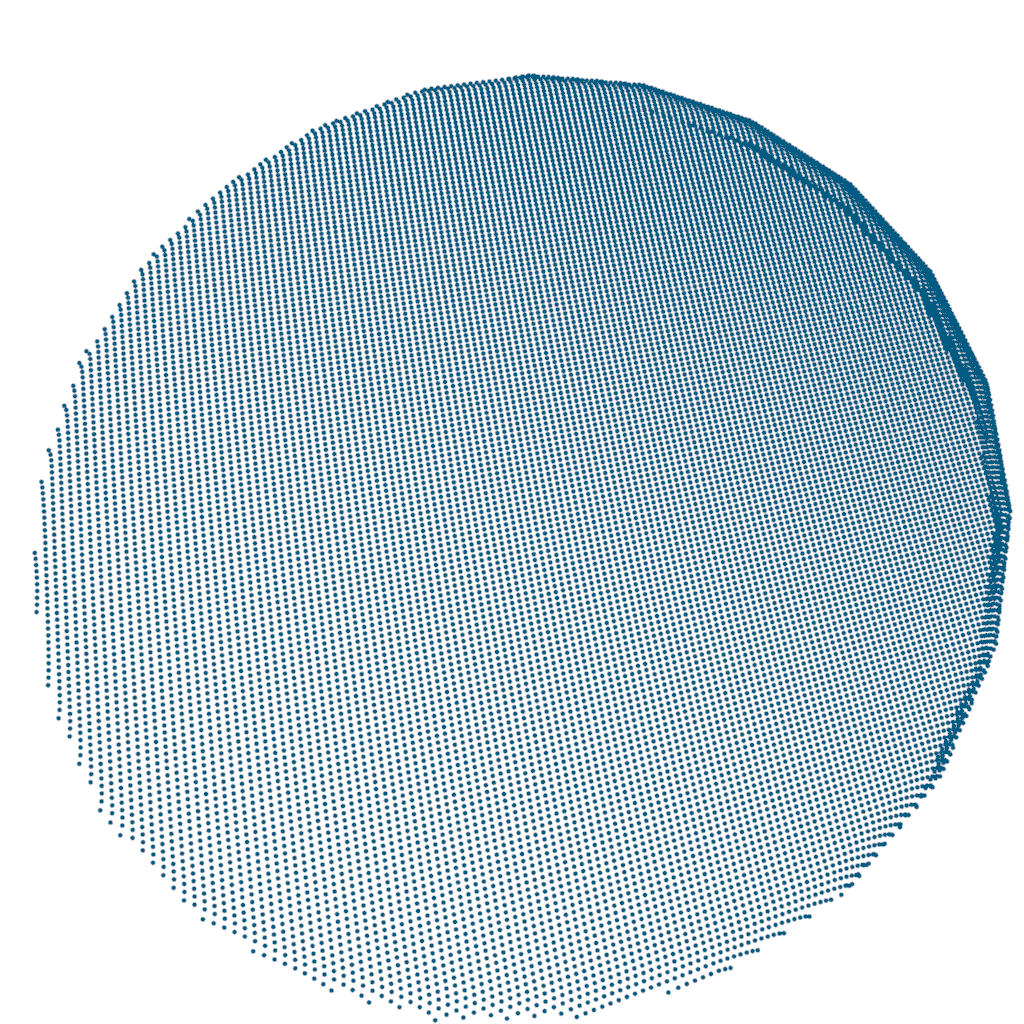
\includegraphics[width=\linewidth]{Figures/ObjRecog/occlusion_0}
		\caption{$\psi=0\%$}
		\label{subfig:objrecog:occlusion:0}
	\end{subfigure}
	\hfill
	\begin{subfigure}{0.32\textwidth}
		\centering
		
\includegraphics[width=\linewidth]{Figures/ObjRecog/occlusion_25}
		\caption{$\psi=25\%$}
		\label{subfig:objrecog:occlusion:25}
	\end{subfigure}
	\hfill
	\begin{subfigure}{0.32\textwidth}
		\centering
		
\includegraphics[width=\linewidth]{Figures/ObjRecog/occlusion_50}
		\caption{$\psi=50\%$}
		\label{subfig:objrecog:occlusion:50}
	\end{subfigure}
	\hfill
	\caption{Different levels of occlusion ($\psi=0\%$ (\subref{subfig:objrecog:occlusion:0}), $\psi=25\%$ (\subref{subfig:objrecog:occlusion:25}), and $\psi=50\%$ (\subref{subfig:objrecog:occlusion:50})) applied randomly to a table partial view.}
	\label{fig:objrecog:occlusion}
\end{figure}

\subsubsection{Implementation and Setup}
\label{cha:objrecog:sec:study:subsec:experiments:subsubsec:setup}

%TODO: Source code

Results were obtained using the following test setup: Intel Core i7-5820K with 32 GiB of Kingston HyperX 2666MHz and CL13 DDR4 RAM on an Asus X99-A motherboard (Intel X99 chipset). Additionally, the system included an NVIDIA Tesla K40c GPU used for training and inference. The framework of choice was Caffe RC2 running on Ubuntu 14.04.02. It was compiled using CMake 2.8.7, g++ 4.8.2, CUDA 7.5, and cuDNN v3.

\subsubsection{Results and Discussion}
\label{cha:objrecog:sec:study:subsec:experiments:subsubsec:results}

The networks were trained for a maximum of $5000$ iterations -- weights were snapshotted every $100$ iterations so in the end we selected the best sets of them as if we were early stopping -- using Adadelta as optimizer with $\delta = 1\cdot10^{-8}$. The regularization term or weight decay in Caffe was set to $5\cdot10^{-3}$. A batch size of $32$ training samples was chosen.

After describing the experimentation setup, the dataset that was used to train and test the networks, and the ways of simulating noise and occlusion for the test sets, we will present and discuss the results of the experiments. Firstly, the normalized density tensor results -- using the \acs{2.5D} \acs{CNN} -- will be presented. After that, we will proceed with the binary tensor ones. Furthermore, we will report the experiments which produced the best results with a pure \acs{3D} \acs{CNN} with fully \acs{3D} convolutions. At last, we will perform a comparison with the state of the art.

\paragraph{Density Tensor}

Figure \ref{fig:objrecog:3dcnn:experiments:25d_density} shows the accuracy results of the network for both grid types and increasing sizes. The peak accuracies for the fixed grids are $\approx0.75$, $\approx0.76$, and $\approx0.73$ for sizes $32$, $48$, and $64$ respectively. In the case of the adaptive one, the peak accuracies are $\approx0.77$, $\approx0.78$, and $\approx0.79$ for the sizes $32$, $48$, and $64$ respectively.

\begin{figure}[!b]
	\centering
	\begin{subfigure}{0.49\textwidth}
		\begin{tikzpicture}
  \begin{axis}[
	  grid=both,
	  width=\linewidth,
	  height=20 em,
      xlabel={Iteration},
      ylabel={Accuracy},
	  legend cell align=left,
      legend pos=south east,
	  legend style={font=\smaller \smaller},
      ymajorgrids=true,
	  y tick style={uablue50},
	  x tick style={uablue50},
      minor grid style={very thin, uagray10},
	  major grid style={uagray10},
	  axis line style={uablue50},
	  ymin=0,
	  ymax=1.0,
	  xmin=0,
	  xmax=5000,
	  restrict x to domain=0:5000,
	  enlarge y limits=true,
	  enlarge x limits=true,
    ]
%
	\addplot [dashed, mark=none, uablue50, line width=0.1 em, smooth] table [col sep=space] {Data/ObjRecog/g32_f_d_training.dat};
	\addplot [mark=none, uablue50, line width=0.1 em, smooth] table [col sep=space] {Data/ObjRecog/g32_f_d_validation.dat};
	\addplot [dashed, mark=none, uabranchblue, line width=0.1 em, smooth] table [col sep=space] {Data/ObjRecog/g48_f_d_training.dat};
	\addplot [mark=none, uabranchblue, line width=0.1 em, smooth] table [col sep=space] {Data/ObjRecog/g48_f_d_validation.dat};
	\addplot [dashed, mark=none, ualightblue, line width=0.1 em, smooth] table [col sep=space] {Data/ObjRecog/g64_f_d_training.dat};
	\addplot [mark=none, ualightblue, line width=0.1 em, smooth] table [col sep=space] {Data/ObjRecog/g64_f_d_validation.dat};
    \legend{g32 (training), g32 (validation), g48 (training), g48 (validation), g64 (training), g64\ (validation)}
  \end{axis}
\end{tikzpicture}

		\caption{Fixed Grid}
		\label{subfig:objrecog:3dcnn:experiments:25d_fixed_density}
	\end{subfigure}
	\begin{subfigure}{0.49\textwidth}
		\begin{tikzpicture}
  \begin{axis}[
	  grid=both,
	  width=\linewidth,
	  height=20 em,
      xlabel={Iteration},
      ylabel={Accuracy},
	  legend cell align=left,
      legend pos=south east,
	  legend style={font=\smaller \smaller},
      ymajorgrids=true,
	  y tick style={uablue50},
	  x tick style={uablue50},
      minor grid style={very thin, uagray10},
	  major grid style={uagray10},
	  axis line style={uablue50},
	  ymin=0,
	  ymax=1.0,
	  xmin=0,
	  xmax=5000,
	  restrict x to domain=0:5000,
	  enlarge y limits=true,
	  enlarge x limits=true,
    ]
%
	\addplot [dashed, mark=none, uablue50, line width=0.1 em, smooth] table [x=iteration, y=acc, col sep=space] {Data/ObjRecog/g32_a_d_training.dat};
	\addplot [mark=none, uablue50, line width=0.1 em, smooth] table [x=iteration, y=acc, col sep=space] {Data/ObjRecog/g32_a_d_validation.dat};
	\addplot [dashed, mark=none, uabranchblue, line width=0.1 em, smooth] table [col sep=space] {Data/ObjRecog/g48_a_d_training.dat};
	\addplot [mark=none, uabranchblue, line width=0.1 em, smooth] table [col sep=space] {Data/ObjRecog/g48_a_d_validation.dat};
	\addplot [dashed, mark=none, ualightblue, line width=0.1 em, smooth] table [col sep=space] {Data/ObjRecog/g64_a_d_training.dat};
	\addplot [mark=none, ualightblue, line width=0.1 em, smooth] table [col sep=space] {Data/ObjRecog/g64_a_d_validation.dat};
    \legend{g32 (training), g32 (validation), g48 (training), g48 (validation), g64 (training), g64 (validation)}
  \end{axis}
\end{tikzpicture}

		\caption{Adaptive Grid}
		\label{subfig:objrecog:3dcnn:experiments:25d_adaptive_density}
	\end{subfigure}
	\caption{Evolution of training and validation accuracy of the model-based \acs{CNN} using both fixed (\subref{subfig:objrecog:3dcnn:experiments:25d_fixed_density}) and adaptive (\subref{subfig:objrecog:3dcnn:experiments:25d_adaptive_density}) normalized density grids. Different grid sizes ($32, 48, $ and $64$) were tested.}
	\label{fig:objrecog:3dcnn:experiments:25d_density}
\end{figure}

Taking those facts into account, we can extract two conclusions. First, the adaptive grid is able to achieve a slightly better peak accuracy in all cases; however, the fixed grid takes less iterations to reach accuracy values close to the peak in all cases. Second, there is no significant difference in using a bigger grid size of $64$ voxels instead of a smaller one of $32$.

The most important fact that can be observed in the aforementioned figures is that there is a considerable gap between training and validation accuracy in all situations. As we can observe, all networks reach maximum accuracy for the training set whilst the validation one hits a glass ceiling at approximately $0.80$. We hypothesize that the network suffers overfitting even when we thoroughly applied measures to avoid that. The most probable cause for that problem is the reduced number of training examples. In the case of ModelNet10 the training set consists of only $3991$ models. Considering the complexity of the \acs{CNN}, it is reasonable to think that the lack of a richer training set is causing overfitting.

\begin{figure}[!b]
	\centering
		\begin{subfigure}{0.49\textwidth}
		\begin{tikzpicture}
  \begin{axis}[
	  grid=both,
	  width=\linewidth,
	  height=20 em,
      xlabel={Occlusion (\%)},
      ylabel={Accuracy},
	  legend cell align=left,
      legend pos=south west,
	  legend style={font=\smaller \smaller},
      ymajorgrids=true,
	  y tick style={uablue50},
	  x tick style={uablue50},
      minor grid style={very thin, uagray10},
	  major grid style={uagray10},
	  axis line style={uablue50},
	  ymin=0,
	  ymax=1.0,
	  xmin=0,
	  xmax=30,
	  restrict x to domain=0:30,
	  enlarge y limits=true,
	  enlarge x limits=true,
    ]
%
	\addplot [mark=none, uablue50, line width=0.1 em, smooth] table [x=percent, y=g32, col sep=space] {Data/ObjRecog/f_d_occlusion.dat};
	\addplot [mark=none, uabranchblue, line width=0.1 em, smooth] table [x=percent, y=g64, col sep=space] {Data/ObjRecog/f_d_occlusion.dat};
	\addplot [mark=none, ualightblue, line width=0.1 em, smooth] table [x=percent, y=g48, col sep=space] {Data/ObjRecog/f_d_occlusion.dat};
    \legend{g32, g48, g64}
  \end{axis}
\end{tikzpicture}

		\caption{Fixed Grid}
		\label{subfig:objrecog:3dcnn:experiments:25d_fixed_density_occlusion}
	\end{subfigure}
	\begin{subfigure}{0.49\textwidth}
		\begin{tikzpicture}
  \begin{axis}[
	  grid=both,
	  width=\linewidth,
	  height=20 em,
      xlabel={Occlusion (\%)},
      ylabel={Accuracy},
	  legend cell align=left,
      legend pos=south west,
	  legend style={font=\smaller \smaller},
      ymajorgrids=true,
	  y tick style={uablue50},
	  x tick style={uablue50},
      minor grid style={very thin, uagray10},
	  major grid style={uagray10},
	  axis line style={uablue50},
	  ymin=0.0,
	  ymax=1.0,
	  xmin=0,
	  xmax=30,
	  restrict x to domain=0:30,
	  enlarge y limits=true,
	  enlarge x limits=true,
    ]
%
	\addplot [mark=none, uablue, line width=0.1 em, smooth] table [x=percent, y=g32, col sep=space] {Data/ObjRecog/a_d_occlusion.dat};
	\addplot [mark=none, uabranchblue, line width=0.1 em, smooth] table [x=percent, y=g48, col sep=space] {Data/ObjRecog/a_d_occlusion.dat};
	\addplot [mark=none, ualightblue, line width=0.1 em, smooth] table [x=percent, y=g64, col sep=space] {Data/ObjRecog/a_d_occlusion.dat};
    \legend{g32, g48, g64}
  \end{axis}
\end{tikzpicture}

		\caption{Adaptive Grid}
		\label{subfig:objrecog:3dcnn:experiments:25d_adaptive_density_occlusion}
	\end{subfigure}
	\caption{Evolution of validation accuracy of the model-based \acs{CNN} using both fixed (\subref{subfig:objrecog:3dcnn:experiments:25d_fixed_density_occlusion}) and adaptive (\subref{subfig:objrecog:3dcnn:experiments:25d_adaptive_density_occlusion}) normalized density grids as the amount of occlusion in the validation models increases from $0\%$ to $30\%$. Three grid sizes were tested ($32, 48, $ and $64$).}
	\label{fig:objrecog:3dcnn:experiments:25d_density_occlusion}
\end{figure}

Concerning the robustness against occlusion, we took the best networks after training and tested them using the same validation sets as before but introducing occlusions in them (up to a $30\%$). Figure \ref{fig:objrecog:3dcnn:experiments:25d_density_occlusion} shows the accuracy of both grid types with different sizes as the amount of occlusion in the validation model increases. As we can observe, occlusion has a significant and negative impact on the fixed grid -- bigger grid sizes are less affected -- going down from $\approx0.75$ accuracy to $0.40 - 0.50$ approximately in the worst and best case respectively when a $30\%$ of the model is occluded. On the contrary, the adaptive grid does not suffer that much -- it goes down from $\approx0.78$ to $\approx0.60$ in the worst case -- and there is no significant difference between grid sizes. In conclusion, the adaptive grid is considerably more robust to occlusion than the fixed one.

Regarding the resilience to noise, we also tested the best networks obtained from the aforementioned training process using validation sets with different levels of noise (ranging from $\sigma=1\cdot10^{-2}$ to $\sigma=1\cdot10^1$). Figure \ref{subfig:objrecog:3dcnn:experiments:25d_adaptive_density_noise} shows the results of those experiments. It can be observed that adding noise has a significant impact on the fixed grid, even small quantities, reducing the accuracy from $\approx0.75$ to $\approx0.60$, $\approx0.4$, and $\approx0.2$ for $\sigma=1\cdot10^{-1}, \sigma=1\cdot{10^0}$, and $\sigma=1\cdot10^1$ respectively. On the other hand, the adaptive one shows remarkable robustness against low levels of noise (up to $\sigma=1\cdot10^{-1}$), barely diminishing its accuracy.

\begin{figure}[!t]
	\centering
	\begin{subfigure}{0.49\textwidth}
		\begin{tikzpicture}
  \begin{axis}[
	  xmode=log,
	  grid=both,
	  width=\linewidth,
	  height=20 em,
      xlabel={Gaussian Noise ($\sigma$)},
      ylabel={Accuracy},
	  legend cell align=left,
      legend pos=south west,
	  legend style={font=\smaller \smaller},
      ymajorgrids=true,
	  y tick style={uablue50},
	  x tick style={uablue50},
      minor grid style={very thin, uagray10},
	  major grid style={uagray10},
	  axis line style={uablue50},
	  ymin=0,
	  ymax=1.0,
	  xmin=0.01,
	  xmax=10,
	  restrict x to domain=:30,
	  enlarge y limits=true,
	  enlarge x limits=true,
    ]
%
	\addplot [mark=none, uablue, line width=0.1 em, smooth] table [x=noise, y=g32, col sep=space] {Data/ObjRecog/f_d_noise.dat};
	\addplot [mark=none, uabranchblue, line width=0.1 em, smooth] table [x=noise, y=g48, col sep=space] {Data/ObjRecog/f_d_noise.dat};
	\addplot [mark=none, ualightblue, line width=0.1 em, smooth] table [x=noise, y=g64, col sep=space] {Data/ObjRecog/f_d_noise.dat};
    \legend{g32, g48, g64}
  \end{axis}
\end{tikzpicture}

		\caption{Fixed Grid}
		\label{subfig:objrecog:3dcnn:experiments:25d_fixed_density_noise}
	\end{subfigure}
	\begin{subfigure}{0.49\textwidth}
		\begin{tikzpicture}
  \begin{axis}[
	  xmode=log,
	  grid=both,
	  width=\linewidth,
	  height=20 em,
      xlabel={Gaussian Noise ($\sigma$)},
      ylabel={Accuracy},
	  legend cell align=left,
      legend pos=south west,
	  legend style={font=\smaller \smaller},
      ymajorgrids=true,
	  y tick style={uablue50},
	  x tick style={uablue50},
      minor grid style={very thin, uagray10},
	  major grid style={uagray10},
	  axis line style={uablue50},
	  ymin=0,
	  ymax=1.0,
	  xmin=0.01,
	  xmax=10,
	  restrict x to domain=:30,
	  enlarge y limits=true,
	  enlarge x limits=true,
    ]
%
	\addplot [mark=none, uablue, line width=0.1 em, smooth] table [x=noise, y=g32, col sep=space] {Data/ObjRecog/a_d_noise.dat};
	\addplot [mark=none, uabranchblue, line width=0.1 em, smooth] table [x=noise, y=g48, col sep=space] {Data/ObjRecog/a_d_noise.dat};
	\addplot [mark=none, ualightblue, line width=0.1 em, smooth] table [x=noise, y=g64, col sep=space] {Data/ObjRecog/a_d_noise.dat};
    \legend{g32, g48, g64}
  \end{axis}
\end{tikzpicture}

		\caption{Adaptive Grid}
		\label{subfig:objrecog:3dcnn:experiments:25d_adaptive_density_noise}
	\end{subfigure}
	\caption{Evolution of validation accuracy of the model-based \acs{CNN} using both fixed (\subref{subfig:objrecog:3dcnn:experiments:25d_fixed_density_noise}) and adaptive (\subref{subfig:objrecog:3dcnn:experiments:25d_adaptive_density_occlusion}) normalized density grids as the standard deviation of the Gaussian noise introduced in the $z$-axis of the views increases from $0.001$ to $10$. The common grid sizes were tested ($32, 48, $ and $64$).}
	\label{fig:objrecog:3dcnn:experiments:25d_density_noise}
\end{figure}

In the end, both grids suffer huge penalties in accuracy when noise levels higher than $\sigma=1\cdot10^-1$ are introduced, being the adaptive one less affected. The grid size has little to no effect in both cases, only in the fixed grid bigger sizes are slightly more robust when intermediate to high levels of noise are introduced. In conclusion, the adaptive grid is significantly more resilient to low levels of noise, and slightly outperforms the fixed one when dealing with intermediate to high ones.

\paragraph{Binary Tensor}

\begin{figure}[!t]
	\centering
	\begin{subfigure}{\textwidth}
		\begin{tikzpicture}
  \begin{axis}[
	  grid=both,
	  width=\linewidth,
	  height=18 em,
      xlabel={Iteration},
      ylabel={Accuracy},
	  legend cell align=left,
      legend pos=south east,
	  legend style={font=\smaller \smaller},
      ymajorgrids=true,
	  y tick style={uablue50},
	ytick={0.0, 0.2, 0.4, 0.6, 0.8, 1.0},
	  x tick style={uablue50},
      minor grid style={very thin, uagray10},
	  major grid style={uagray10},
	  axis line style={uablue50},
	  ymin=0,
	  ymax=1.0,
	 xtick={0, 1000, 2000, 3000, 4000, 5000},
	  xmin=0,
	  xmax=5000,
	  restrict x to domain=0:5000,
	  enlarge y limits=true,
	  enlarge x limits=true,
    ]
%
	\addplot [dashed, mark=none, uablue, line width=0.1 em, smooth] table [col sep=space] {Data/ObjRecog/g32_a_b_training.dat};
	\addplot [, mark=none, uablue, line width=0.1 em, smooth] table [col sep=space] {Data/ObjRecog/g32_a_b_validation.dat};
	\addplot [dashed, mark=none, ualightblue, line width=0.1 em, smooth] table [col sep=space] {Data/ObjRecog/g64_a_b_training.dat};
	\addplot [, mark=none, ualightblue, line width=0.1 em, smooth] table [col sep=space] {Data/ObjRecog/g64_a_b_validation.dat};
    \legend{g32 (training), g32 (validation),  g64 (training), g64\ (validation)}
  \end{axis}
\end{tikzpicture}

		\caption{Training}
		\label{subfig:objrecog:3dcnn:experiments:25d_adaptive_binary}
	\end{subfigure}
	\centering
	\par\bigskip
	\begin{subfigure}{0.49\linewidth}
		\begin{tikzpicture}
  \begin{axis}[
	  grid=both,
	  width=\linewidth,
	  height=18 em,
      xlabel={Occlusion (\%)},
      ylabel={Accuracy},
	  legend cell align=left,
      legend pos=south west,
	  legend style={font=\smaller \smaller},
      ymajorgrids=true,
	  y tick style={uablue50},
	ytick={0.0, 0.2, 0.4, 0.6, 0.8, 1.0},
	  x tick style={uablue50},
      minor grid style={very thin, uagray10},
	  major grid style={uagray10},
	  axis line style={uablue50},
	  ymin=0,
	  ymax=1.0,
	  xmin=0,
	  xmax=30,
	  restrict x to domain=0:30,
	  enlarge y limits=true,
	  enlarge x limits=true,
    ]
%
	\addplot [mark=none, uablue, line width=0.1 em, smooth] table [x=percent, y=g32, col sep=space] {Data/ObjRecog/a_b_occlusion.dat};
	\addplot [mark=none, ualightblue, line width=0.1 em, smooth] table [x=percent, y=g64, col sep=space] {Data/ObjRecog/a_b_occlusion.dat};
    \legend{g32,g64}
  \end{axis}
\end{tikzpicture}

		\caption{Occlusion}
		\label{subfig:objrecog:3dcnn:experiments:25d_adaptive_binary_occlusion}
	\end{subfigure}
	\hfill
	\begin{subfigure}{0.49\linewidth}
		\begin{tikzpicture}
  \begin{axis}[
	  xmode=log,
	  grid=both,
	  width=\linewidth,
	  height=18 em,
      xlabel={Gaussian Noise ($\sigma$)},
      ylabel={Accuracy},
	  legend cell align=left,
      legend pos=south west,
	  legend style={font=\smaller \smaller},
      ymajorgrids=true,
	  y tick style={uablue50},
	ytick={0.0, 0.2, 0.4, 0.6, 0.8, 1.0},
	  x tick style={uablue50},
      minor grid style={very thin, uagray10},
	  major grid style={uagray10},
	  axis line style={uablue50},
	  ymin=0,
	  ymax=1.0,
	  xmin=0.01,
	  xmax=10,
	  restrict x to domain=:30,
	  enlarge y limits=true,
	  enlarge x limits=true,
    ]
%
	\addplot [mark=none, uablue, line width=0.1 em, smooth] table [x=noise, y=g32, col sep=space] {Data/ObjRecog/a_b_noise.dat};
	\addplot [mark=none, ualightblue, line width=0.1 em, smooth] table [x=noise, y=g64, col sep=space] {Data/ObjRecog/a_b_noise.dat};
    \legend{g32, g64}
  \end{axis}
\end{tikzpicture}

		\caption{Noise}
		\label{subfig:objrecog:3dcnn:experiments:25d_adaptive_binary_noise}
	\end{subfigure}
	\caption{Evolution of training and validation accuracy of the model-based \acs{CNN} using adaptive binary grids (\subref{subfig:objrecog:3dcnn:experiments:25d_adaptive_binary}). Evolution of validation accuracy for the best network weights after training as the amount of occlusion in the validation set increases (\subref{subfig:objrecog:3dcnn:experiments:25d_adaptive_binary_occlusion}) and different levels of noise are introduced (\subref{subfig:objrecog:3dcnn:experiments:25d_adaptive_binary_noise}).}
	\label{fig:objrecog:3dcnn:experiments:25d_binary}
\end{figure}

After testing the performance of the normalized density grid, we also trained and assessed the accuracy of the binary one in the same scenarios. This test intended to show whether there is any gain in using representations which include more information about the shape -- at a small penalty to execution time.

For this experimentation we picked the best performer in the previous sections: the adaptive grid. We also discarded the intermediate size ($48$ voxels) since there was no significant difference between it and the others. Figure \ref{fig:objrecog:3dcnn:experiments:25d_adaptive_binary} shows the accuracy results of the network trained using binary grids. As we can observe, there is no significant difference between grid sizes neither. However, using this representation we achieved a peak accuracy of approximately $0.85$, using $64$ voxels grids, which is better to some extent than the normalized density one shown in Figure \ref{fig:objrecog:3dcnn:experiments:25d_density}.

Occlusion and noise tolerance (shown in Figures \ref{subfig:objrecog:3dcnn:experiments:25d_adaptive_binary_occlusion} and \ref{subfig:objrecog:3dcnn:experiments:25d_adaptive_binary_noise} respectively) is mostly similar to the robustness shown by the normalized density adaptive grid (see Figures \ref{subfig:objrecog:3dcnn:experiments:25d_adaptive_density_occlusion} and \ref{subfig:objrecog:3dcnn:experiments:25d_adaptive_density_noise}) except from a small offset caused by the higher accuracy of the binary grid network.

In conclusion, the less-is-better effect applies in this situation and turns out that the simplification introduced by the binary representation helps the network during the learning process. It is pending to check if this statement is still valid if the validation accuracy is not bounded by network overfitting.

\paragraph{3D \ac{CNN}}

At last, we tested the best configuration -- binary adaptive grids -- with a \acs{3D} \acs{CNN} architecture with pure \acs{3D} convolutions. We kept the same architecture we introduced in Section \ref{sec:convolutional_neural_network}, but extended its convolution and pooling layers to three dimensions. We then trained the network using adaptive binary grids as the volumetric representation of choice and monitored validation and training errors. Due to memory limitations on the \acs{GPU} we could only experiment with grids of $32\times32\times32$ voxels.

\begin{figure}[!hbt]
	\centering
	\begin{tikzpicture}
  \begin{axis}[
	  grid=both,
	  width=\linewidth,
	  height=22 em,
      xlabel={Iteration},
      ylabel={Accuracy},
	  legend cell align=left,
      legend pos=south east,
	  legend style={font=\smaller \smaller},
      ymajorgrids=true,
	  y tick style={uablue50},
	  x tick style={uablue50},
      minor grid style={very thin, uagray10},
	  major grid style={uagray10},
	  axis line style={uablue50},
	  ymin=0,
	  ymax=1.0,
	  xmin=0,
	  xmax=25000,
	  xtick={0, 5000, 10000, 15000, 20000, 25000},
	  restrict x to domain=0:25000,
	  enlarge y limits=true,
	  enlarge x limits=true,
    ]
%
	\addplot [dashed, mark=none, uablue, line width=0.1 em, smooth] table [x=iteration, y=acc, col sep=space] {Data/ObjRecog/3d_g32_a_d_training.dat};
	\addplot [mark=none, uablue, line width=0.1 em, smooth] table [x=iteration, y=acc, col sep=space] {Data/ObjRecog/3d_g32_a_d_validation.dat};
    \legend{g32(training), g32(validation)}
  \end{axis}
\end{tikzpicture}

	\caption{Evolution of training and validation accuracy of the \acs{3D} \acs{CNN} using adaptive binary grids with size $32\times32\times32$.}
	\label{fig:objrecog:3dcnn:experiments:3d}
\end{figure}

\newpage

Figure \ref{fig:objrecog:3dcnn:experiments:3d} shows the results of this experiment. As we can observe, we trained the network for five times more iterations than before and even then we couldn't achieve a proper convergence. The training set accuracy kept increasing slowly up to approximately $0.65$ whilst the validation one got stuck around $0.40$ for the whole experiment.

In conclusion, porting the \acs{2.5D} network directly to \acs{3D} just by extending its convolution and pooling layers to slide along the depth axis did not produce good results using the same dataset and setup that produced a significantly good outcome with the \acs{2.5D} architecture. We hypothesize various causes for this problem.

On the one hand, the data representation might not be adequate for such fine-grained convolutions. It is presumable that bigger grids, e.g., $64\times64\times64$, would yield better results. However, given the size of the model, they could not be tested in the available GPU.

On the other hand, the complexity of the network increased considerably after including that extra dimension in convolution and pooling layers. This means that the number of parameters of the network gets increased significantly, making it harder to train with so few samples due to overfitting. This hypothesis is backed up by the fact that training accuracy kept increasing slowly while validation one got stuck. This would eventually lead to a perfect fit on the training set but low accuracy on the validation split.

\paragraph{Discussion}

To sum up, we determined that the adaptive grid slightly outperforms the fixed one in normal conditions. The same happens with the grid size, obtaining marginally better results with bigger sizes. However, when it comes down to noise and occlusion robustness, the adaptive grid exceeds the accuracy of the fixed grid by a large margin for low levels of occlusion and noise, whilst for intermediate and high levels the impact on both grids is somewhat similar. In other words, the adaptive grid is better than the fixed one and it is preferable to use a bigger grid size if the performance impact can be afforded.

It is important to remark that the binary occupancy measure performed better than the normalized density one, both using adaptive grids, while maintaining similar resilience against noise and occlusions. The best network trained with normalized density grids reached a peak accuracy of approximately 0.79 while the best binary one achieved approximately a 0.85 accuracy on the validation set.

Another remarkable fact was that all networks exhibited a considerable amount of overfitting, i.e., training accuracy was almost perfect whilst validation was far away from it by a considerable margin. We hypothesize that this was due to the fact that the dataset has few training examples considering the complexity of the network. Besides, we also inspected the confusion matrix shown in Table \ref{table:confmatrix} to gain insight about the behavior of our network. As we can observe, there are many misclassified samples of classes that are similar. If we take a closer look at some of the misclassified samples (see Figures \ref{fig:3dcnn:experiments:confusion_desk_table}, \ref{fig:3dcnn:experiments:confusion_nstand_dresser}, and \ref{fig:3dcnn:experiments:confusion_sofa_bed}) it is reasonable to think that the network is not able to classify them properly because they are extremely similar. In this regard, the dataset must be augmented introducing noise, translations, rotations, and variations of the models to avoid overfitting and learn better those models that can be easily misclassified.

\subsection{Conclusion}
\label{cha:objrecog:sec:study:subsec:conclusion}

\section{LonchaNet}
\label{cha:objrecog:sec:lonchanet}

\section{Conclusion}
\label{cha:objrecog:sec:conclusion}
